\section{設計概要}
\subsection{初期サンプル}
前章では最もベーシックなrf-SQUID型の結合回路について解説した。本研究の初期段階においても先行研究に倣い単純なrf-SQUID型の結合回路を作成することから始めた。
\begin{figure}[H]
    \centering
    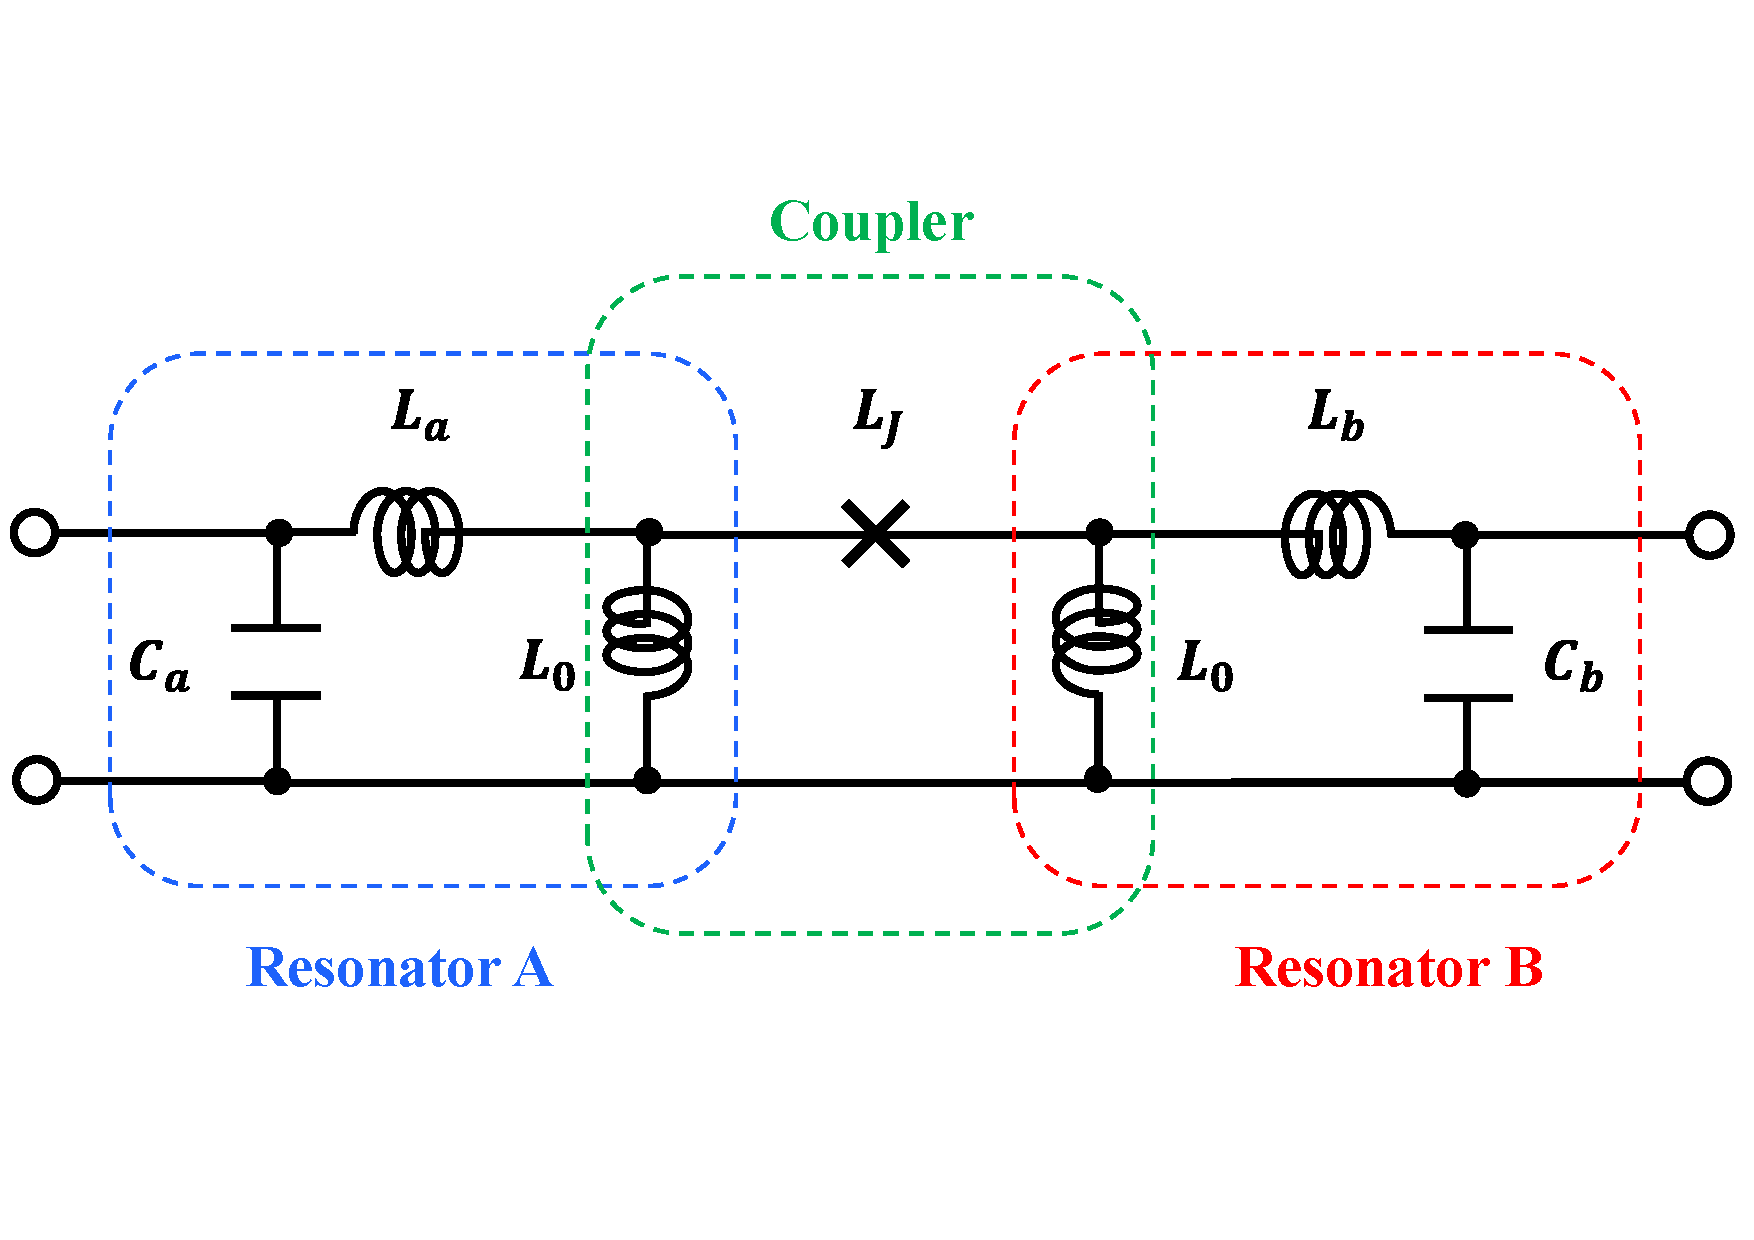
\includegraphics[width=12cm]{theory_circuit1_1.pdf}
    \caption{LEAl}
\end{figure}
作成したサンプルはそれぞれCPW型の共振器、LE型共振器の2つを採用した。また、CPW型共振器には超伝導ループとしてNb(ジョセフソン接合はAl)をLE型についてはNbで作成したものAlで作成したものの2パターンを作成した。それぞれCPWNb,LENb,LEAlとラベリングする。\\
測定結果については測定の章で詳細に記述するが、この3タイプのサンプルのうち有意な結果が得られたのはLEAlであった。よって本章ではLEAlをベースに結合性能の向上にむけて採用したアプローチを中心に解説する。\\
\subsection{中期サンプル}
前章で解説したように結合強度を決定するのはrf-SQUIDを介した実効相互インダクタンス$M_{eff}$と共振器間の磁気的1次結合$M_{ab}$の和である。このうち$M_{ab}$は距離に強く依存する。
\begin{equation}
    M_{eff}(\Phi)  = \frac{L_0^2}{L_{rf}(\Phi)}=\frac{L_0^2}{L_{S}} \frac{\beta \cos \left(2 \pi \Phi/\phi_{0}\right)}{1+\beta \cos \left(2 \pi \Phi/\phi_{0}\right)}
\end{equation}
$M_{eff}$の強度増強を試みる場合考えられる方法は大きく2つ
\begin{enumerate}
    \item rf-SQUID間と共振器の相互インダクタンス$L_0$の強度を増強する
    \item rf-SQUIDのスクリーニングパラメータ$\beta$を限りなく1に近づける
 \end{enumerate}
このうち、まずはrf-SQUID間と共振器の相互インダクタンス$L_0$の強度を増強することを第1に考えた。理由はスクリーニングパラメータを$\beta<1$を満たしつつ限りなく1に漸近させることが設計上困難なためである。$\beta$が1を超えてしまうとrf-SQUIDを貫く磁束は外部磁束に対して2価の関数になると同時にポテンシャルの安定点はループを貫く磁束に対してダブルポテンシャルをとるようになる。共振器間の安定な結合を得るには$\beta<1$は必ず満たさなければならない条件である。
\begin{figure}[H]
    \begin{minipage}[t]{0.5\columnwidth}
        \centering
        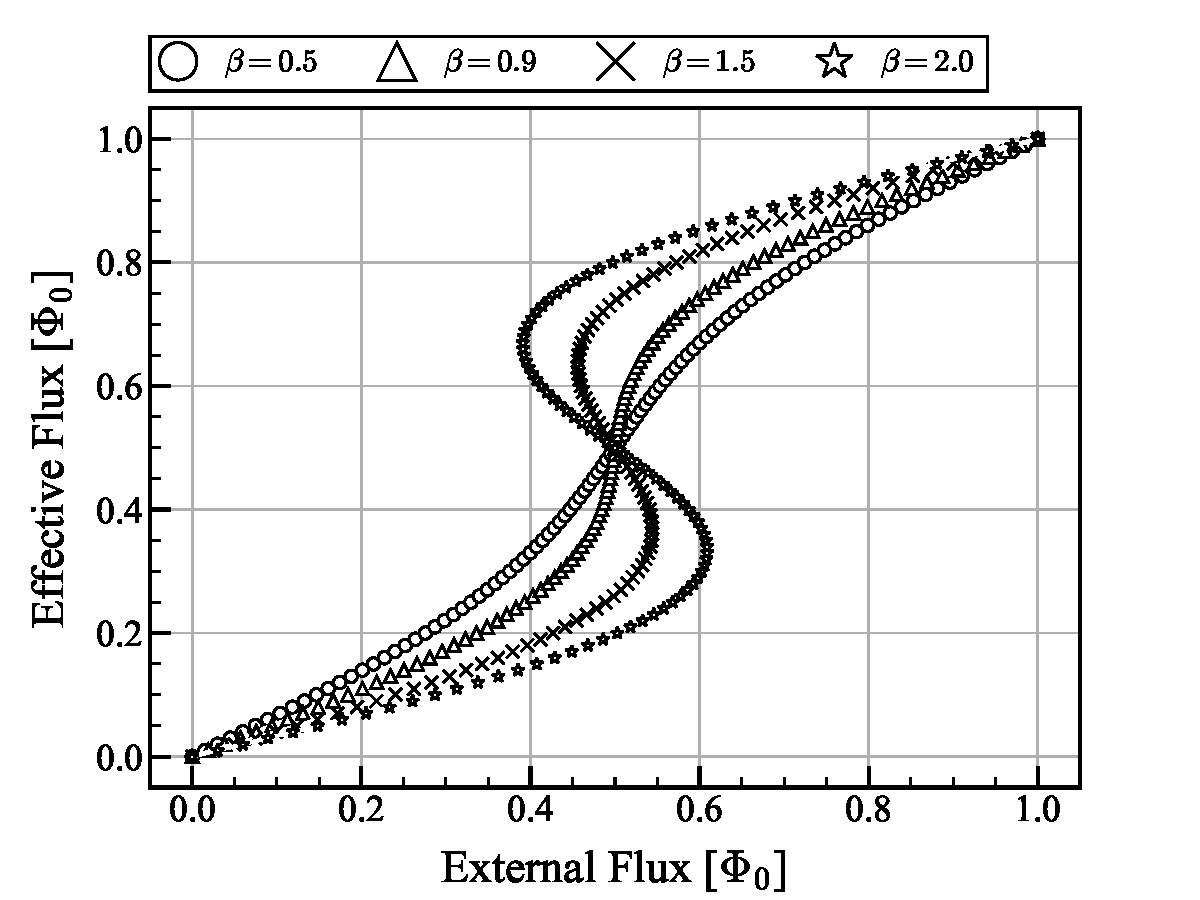
\includegraphics[clip, width=1.0\columnwidth]{rfsquid_current.pdf}
        \caption{外部磁束に対する実効磁束の挙動の変化}
    \end{minipage}%
    \begin{minipage}[t]{0.5\columnwidth}
        \centering
        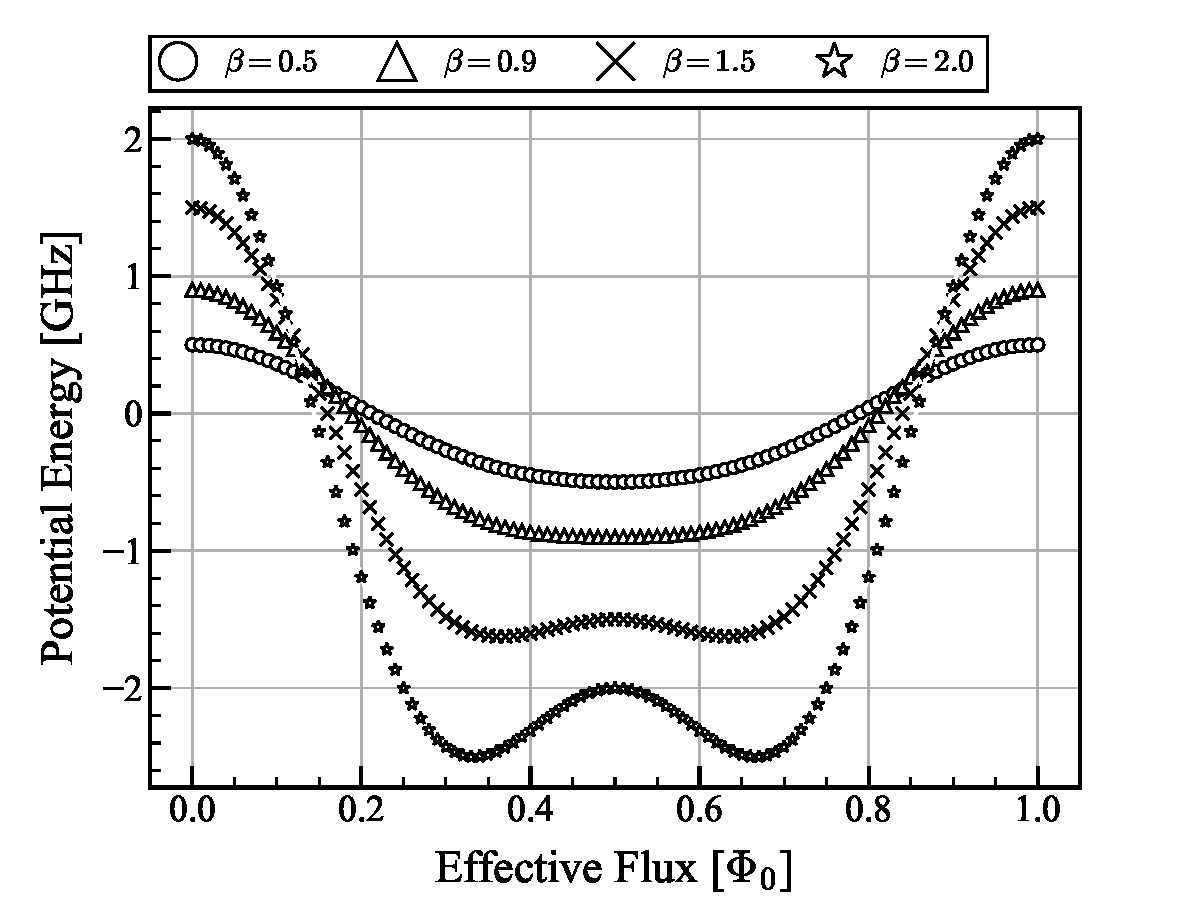
\includegraphics[clip, width=1.0\columnwidth]{rfsquid_potential.pdf}
        \caption{実効磁束に対するポテンシャルエネルギーの挙動の変化}
    \end{minipage}
\end{figure}
本研究においてはrf-SQUIDと共振器間の自己インダクタンス$L_0$を強めるためにガルバニック結合を採用している。そこでさらなる自己インダクタンスの増強に向けてジョセフソン接合をガルバニック結合に付与することを考えた。ガルバニック結合にジョセフソン接合を採用する事例は共振器と磁束量子ビットの深強結合等の先行研究\cite*{Yoshihara2017}があり、これに倣った形である。先行研究ではさらにジョセフソン接合をdc-SQUIDに置き換えることで強力な結合強度を得ることに成功している。
本研究では自己インダクタンス$L_0$をジョセフソンインダクタンス$L_J$で置き換える形で回路を作成した。このサンプルを以下LEJとラベリングする。LEJの設計は伊藤氏、鈴木氏の仕事である。
\begin{figure}[H]
    \centering
    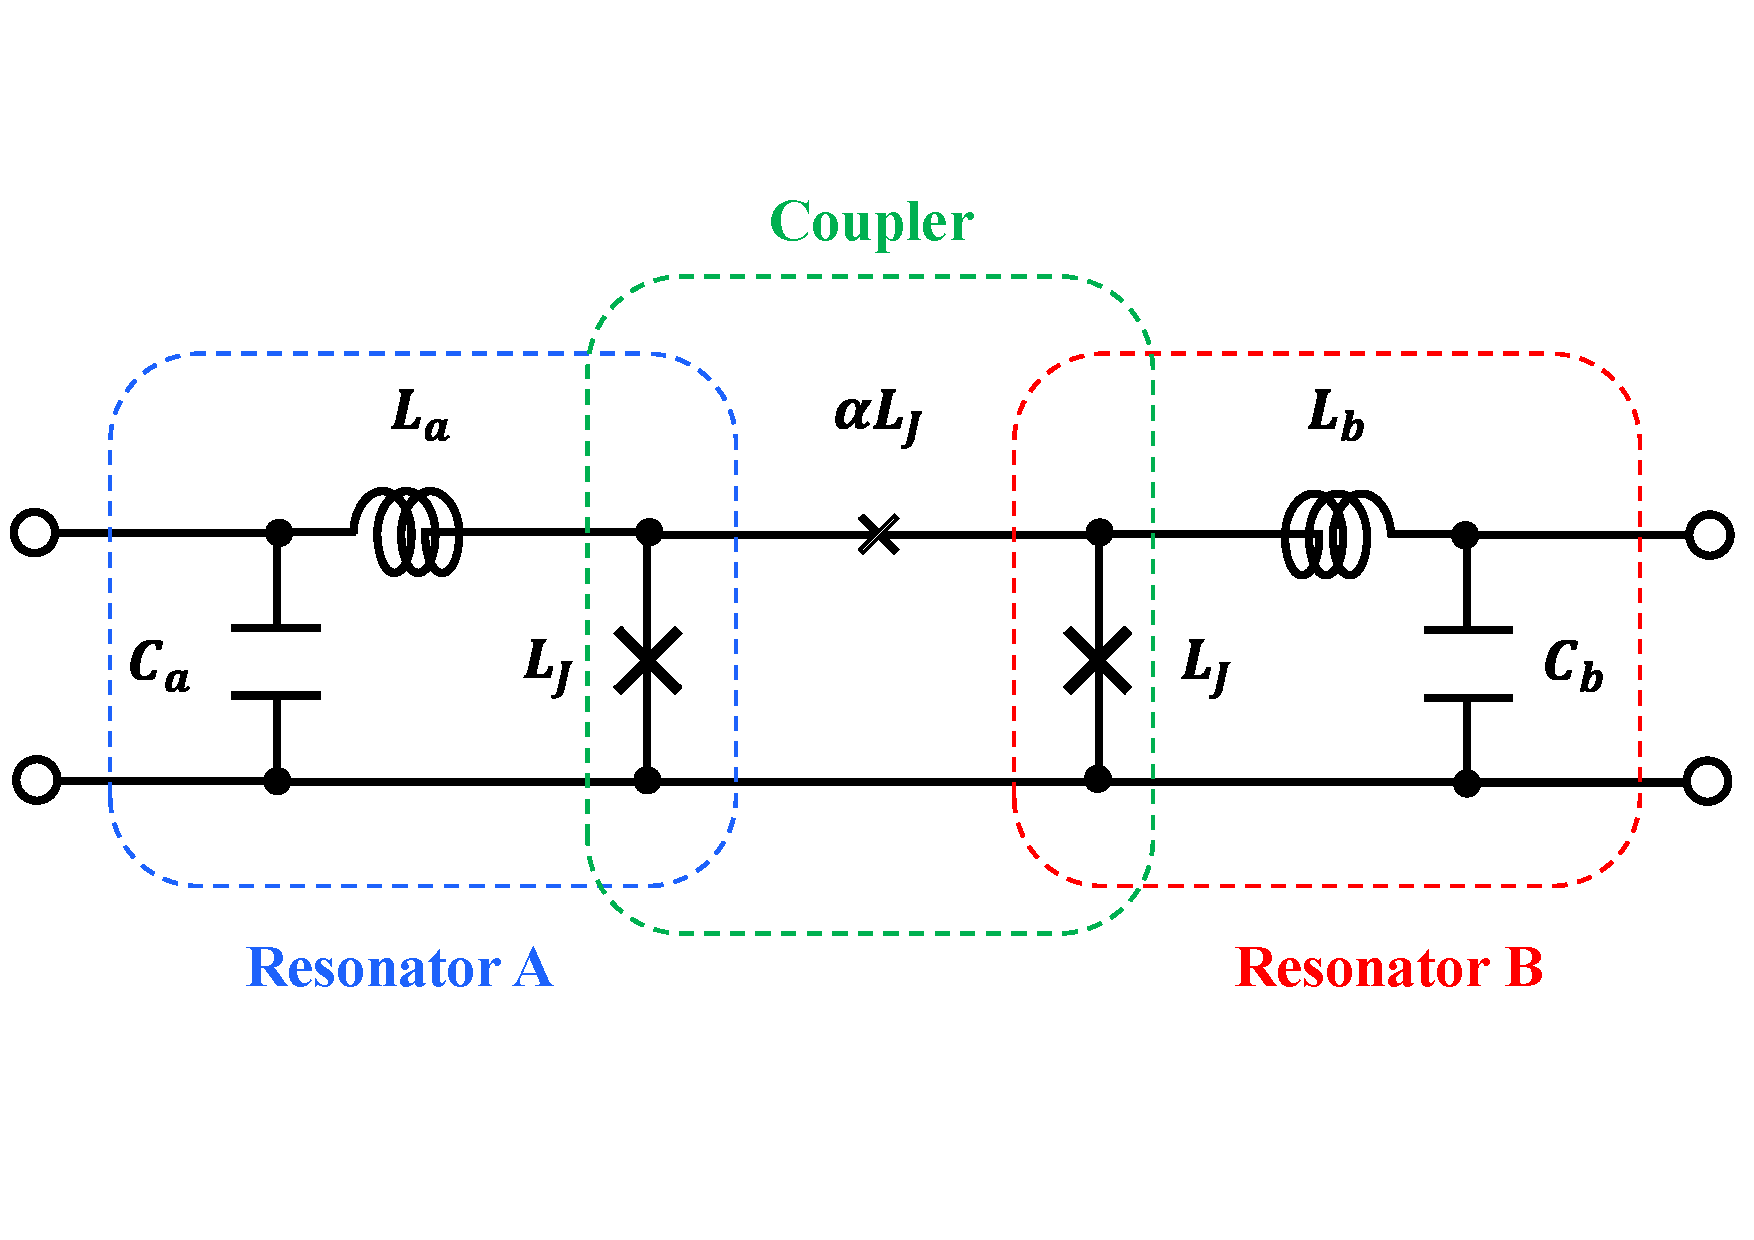
\includegraphics[width=12cm]{theory_circuit2_1.pdf}
    \caption{LEJ}
\end{figure}
\subsection{後期サンプル}
サンプルの詳細な結果については次章で解説するが結果のみ述べればLEAlと比較して正方向に於ける結合強度が増強し、負方向に於ける結合強度は減少した。
この結果についてそれぞれ考えられる理由としては
\begin{enumerate}
    \item $L_J$の追加によって$L_0$が実効的に増加した
    \item ループサイズがLEAlよりも小さいこと
    \item rf-SQUIDのスクリーニングパラメータのが設計通りにならなかったこと
 \end{enumerate}
 等が考えられる。\\
 ジョセフソン接合を追加することによって自己インダクタンスを増強することができた一方で、測定したスペクトルにはLEAlでは観測されなかった非線形な作用が生じた。これは結合素子として扱うには回路自体を複雑にしてしまうため、望ましくない。また、rf-SQUID-共振器間の自己インダクタンス$L_0$がいくら大きくとも、rf-SQUIDのスクリーニングパラメータ$\beta$が適切な値にならなければ高強度な結合は得られない。逆に、緻密にスクリーニングパラメータを決定することができれば非常に高強度な結合を得ることができる。
 \begin{figure}[H]
    \begin{minipage}[t]{0.5\columnwidth}
        \centering
        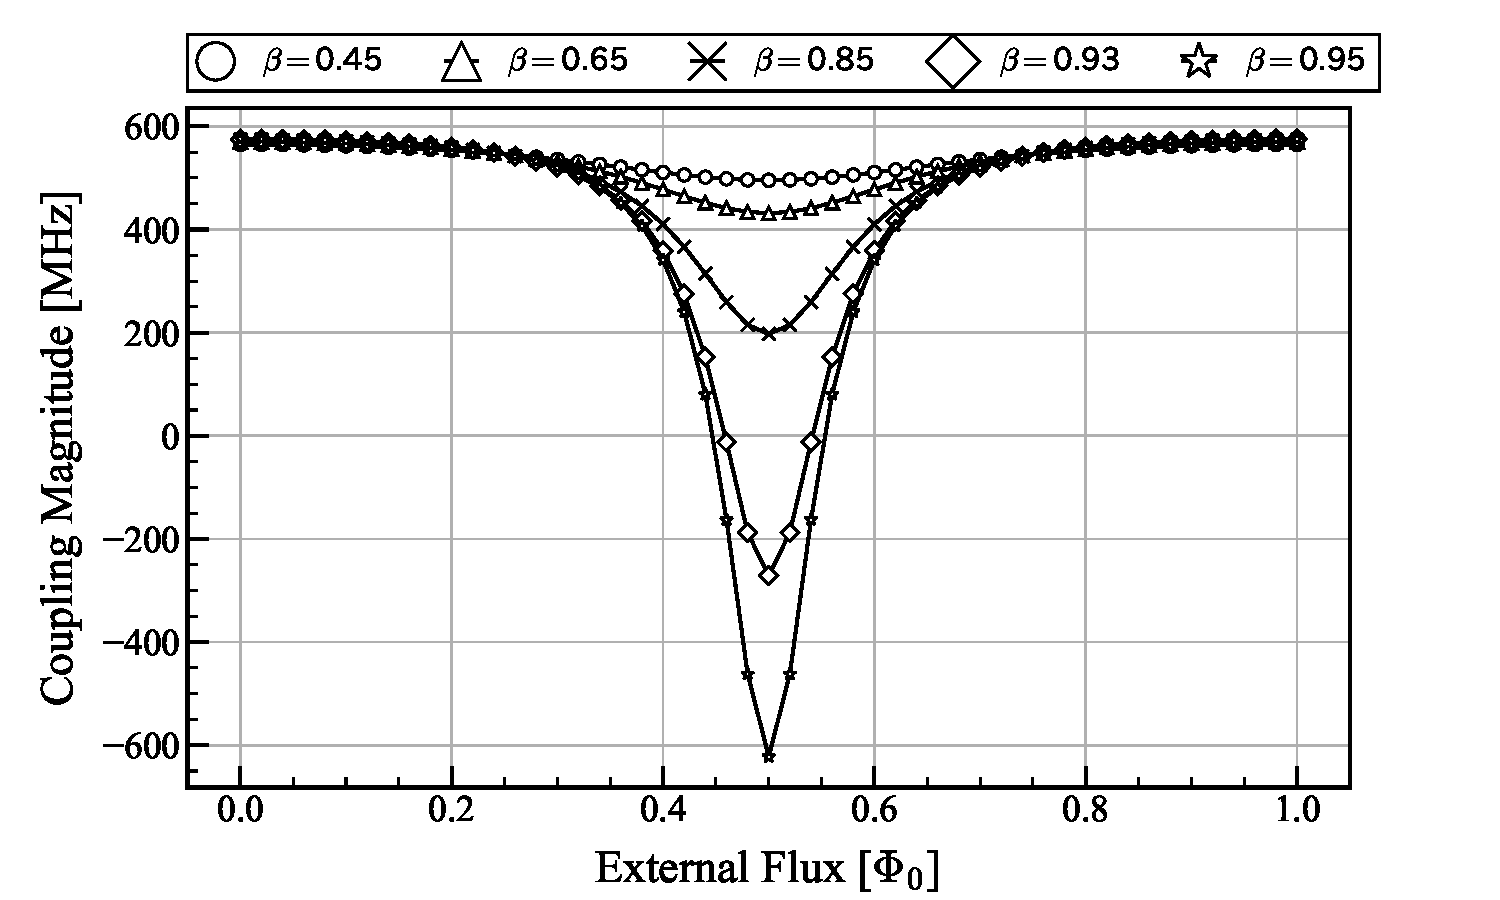
\includegraphics[clip, width=1.0\columnwidth]{standard_coupling_beta.pdf}
        \caption{結合強度の$\beta$依存性}
    \end{minipage}%
    \begin{minipage}[t]{0.5\columnwidth}
        \centering
        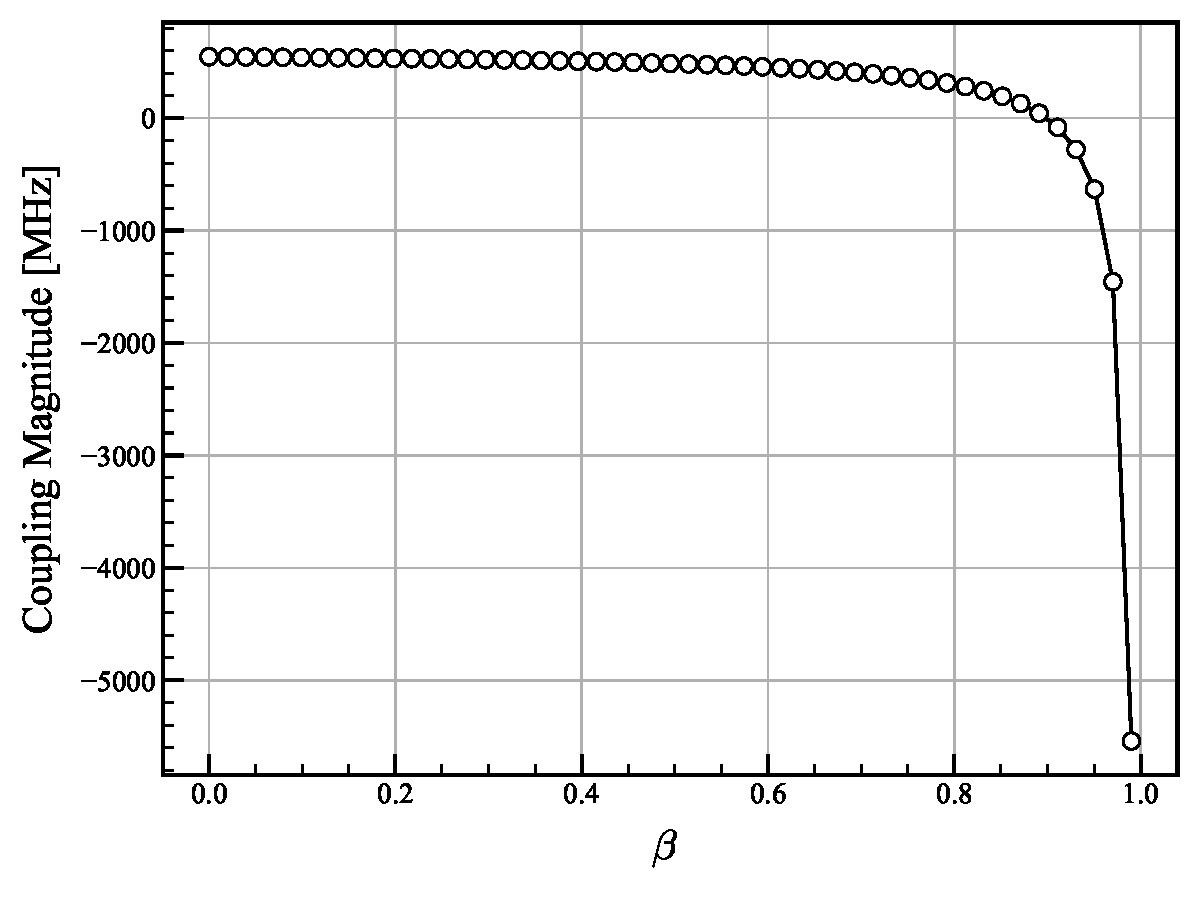
\includegraphics[clip, width=1.0\columnwidth]{standard_coupling_betasweep.pdf}
        \caption{外部磁束を最適動作点に固定した状態での$\beta$依存性}
    \end{minipage}
\end{figure}
 ここまでの結果から考慮すべき点をまとめると
 \begin{enumerate}
    \item ジョセフソン接合を用いずに高強度な自己インダクタンス$L_0$を達成すること
    \item ループの形状は共振器に対して縦長な構造をとることで、共振器間距離を狭めること
    \item rf-SQDUIのスクリーニングパラメータ$\beta$を適切に製作できるような設計にすること
 \end{enumerate}
本研究において上記の条件を達成するためにとった手法は
\begin{enumerate}
    \item rf-SQUID-共振器間の自己インダクタンスにミアンダインダクタンスを導入
    \item 測定時にスクリーニングパラメータ$\beta$を決定できるようにdc-SQUIDを導入
 \end{enumerate}
 である。このミアンダインダクタンスを追加したサンプルを以下LEMとラベリングする。
 \begin{figure}[H]
    \centering
    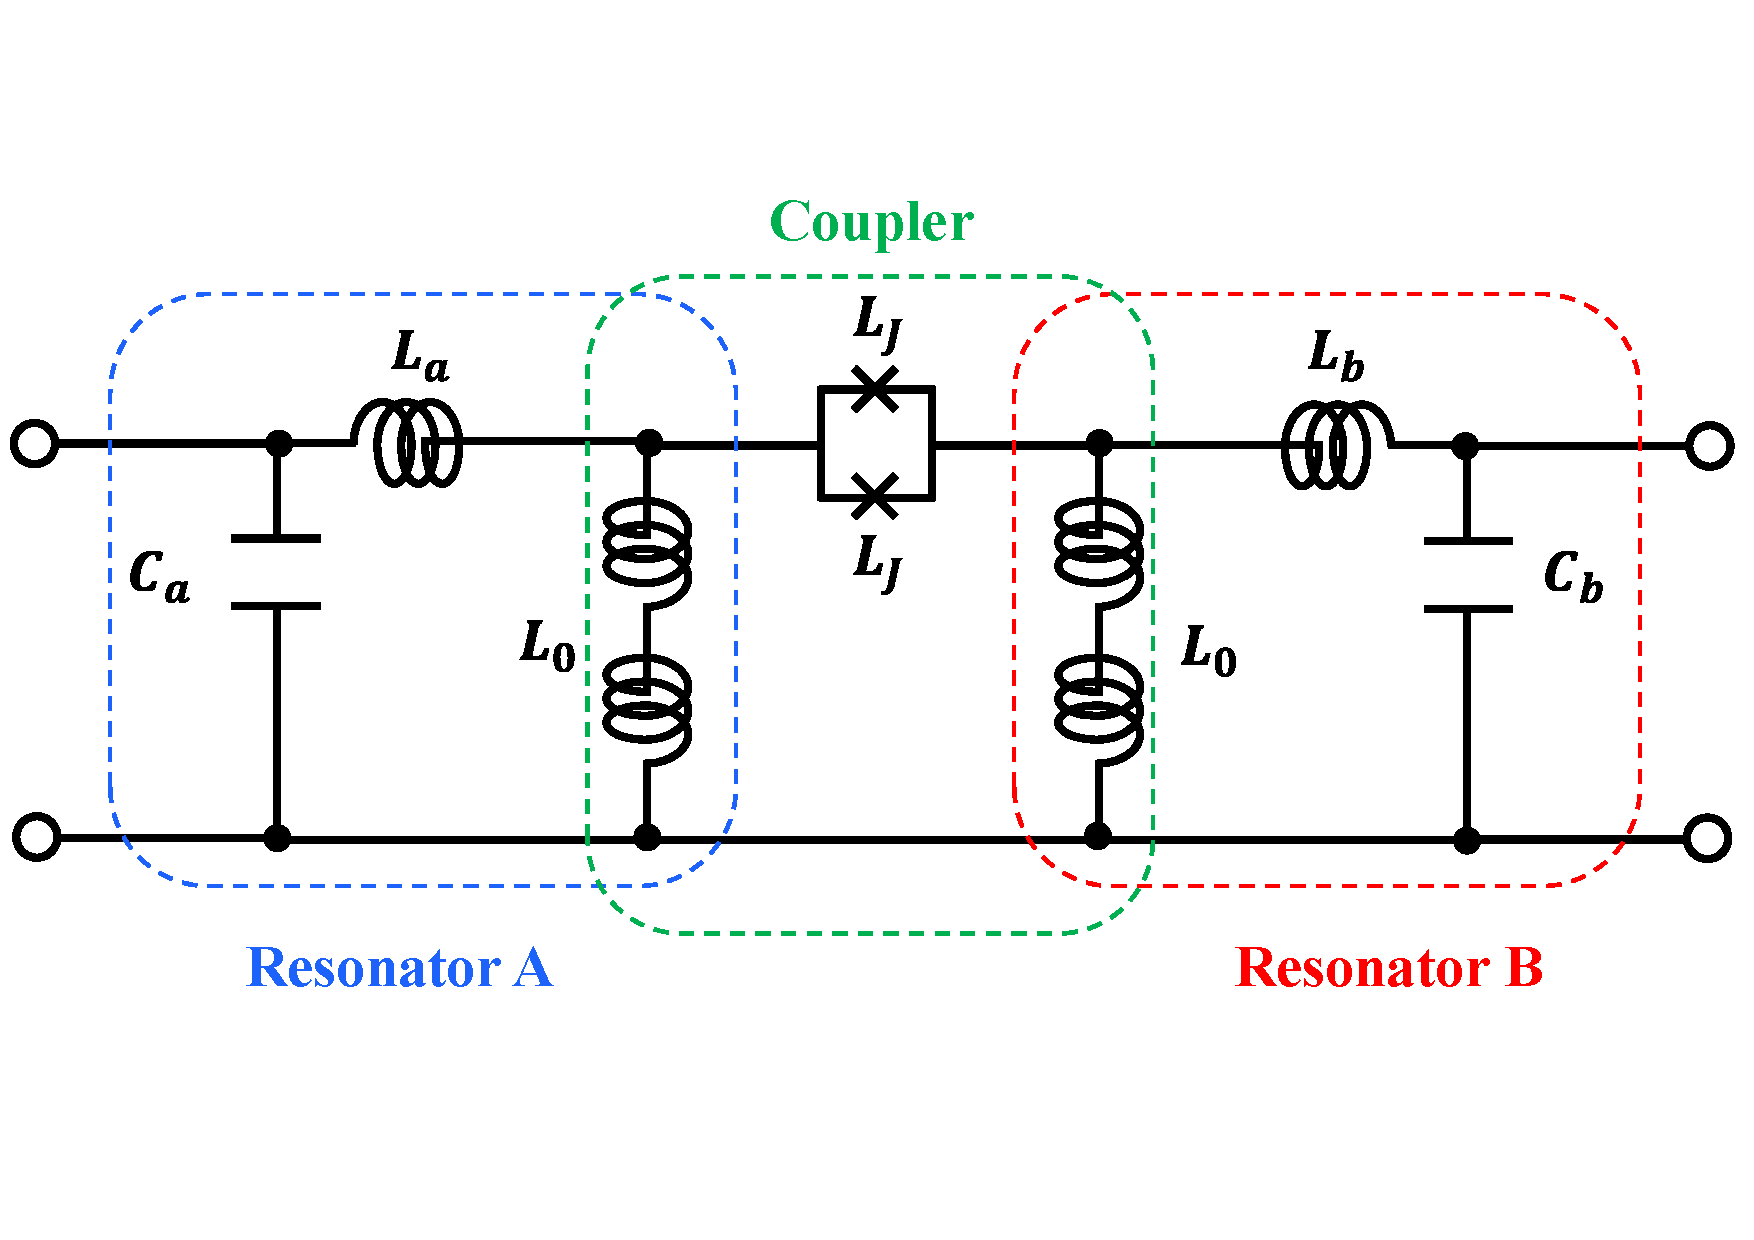
\includegraphics[width=12cm]{theory_circuit3_1.pdf}
    \caption{LEM}
\end{figure}
ミアンダインダクタンスについては既に前章で解説したため、ここではジョセフソン接合の代わりにrf-SQUIDを用いることでスクリーニングパラメータの変調が可能となることを以下に示す。\\
LEMの回路図中結合素子部分のみに注目した図について
    %     今回測定したサンプルは3つである。作成時期順に列挙すると、基本形となるrf-SQUIDを共振器間に配置したLCC。そしてrf-SQUIDと共振器間の結合部にジョセフソン接合を導入したJLCC、最後に接合部をミアンダインダクタンスに変更したMLCCである。まずは基本型の構造は先行論文がとっている手法と全く同じである。
    %     \begin{figure}[H]
    %         \centering
    %         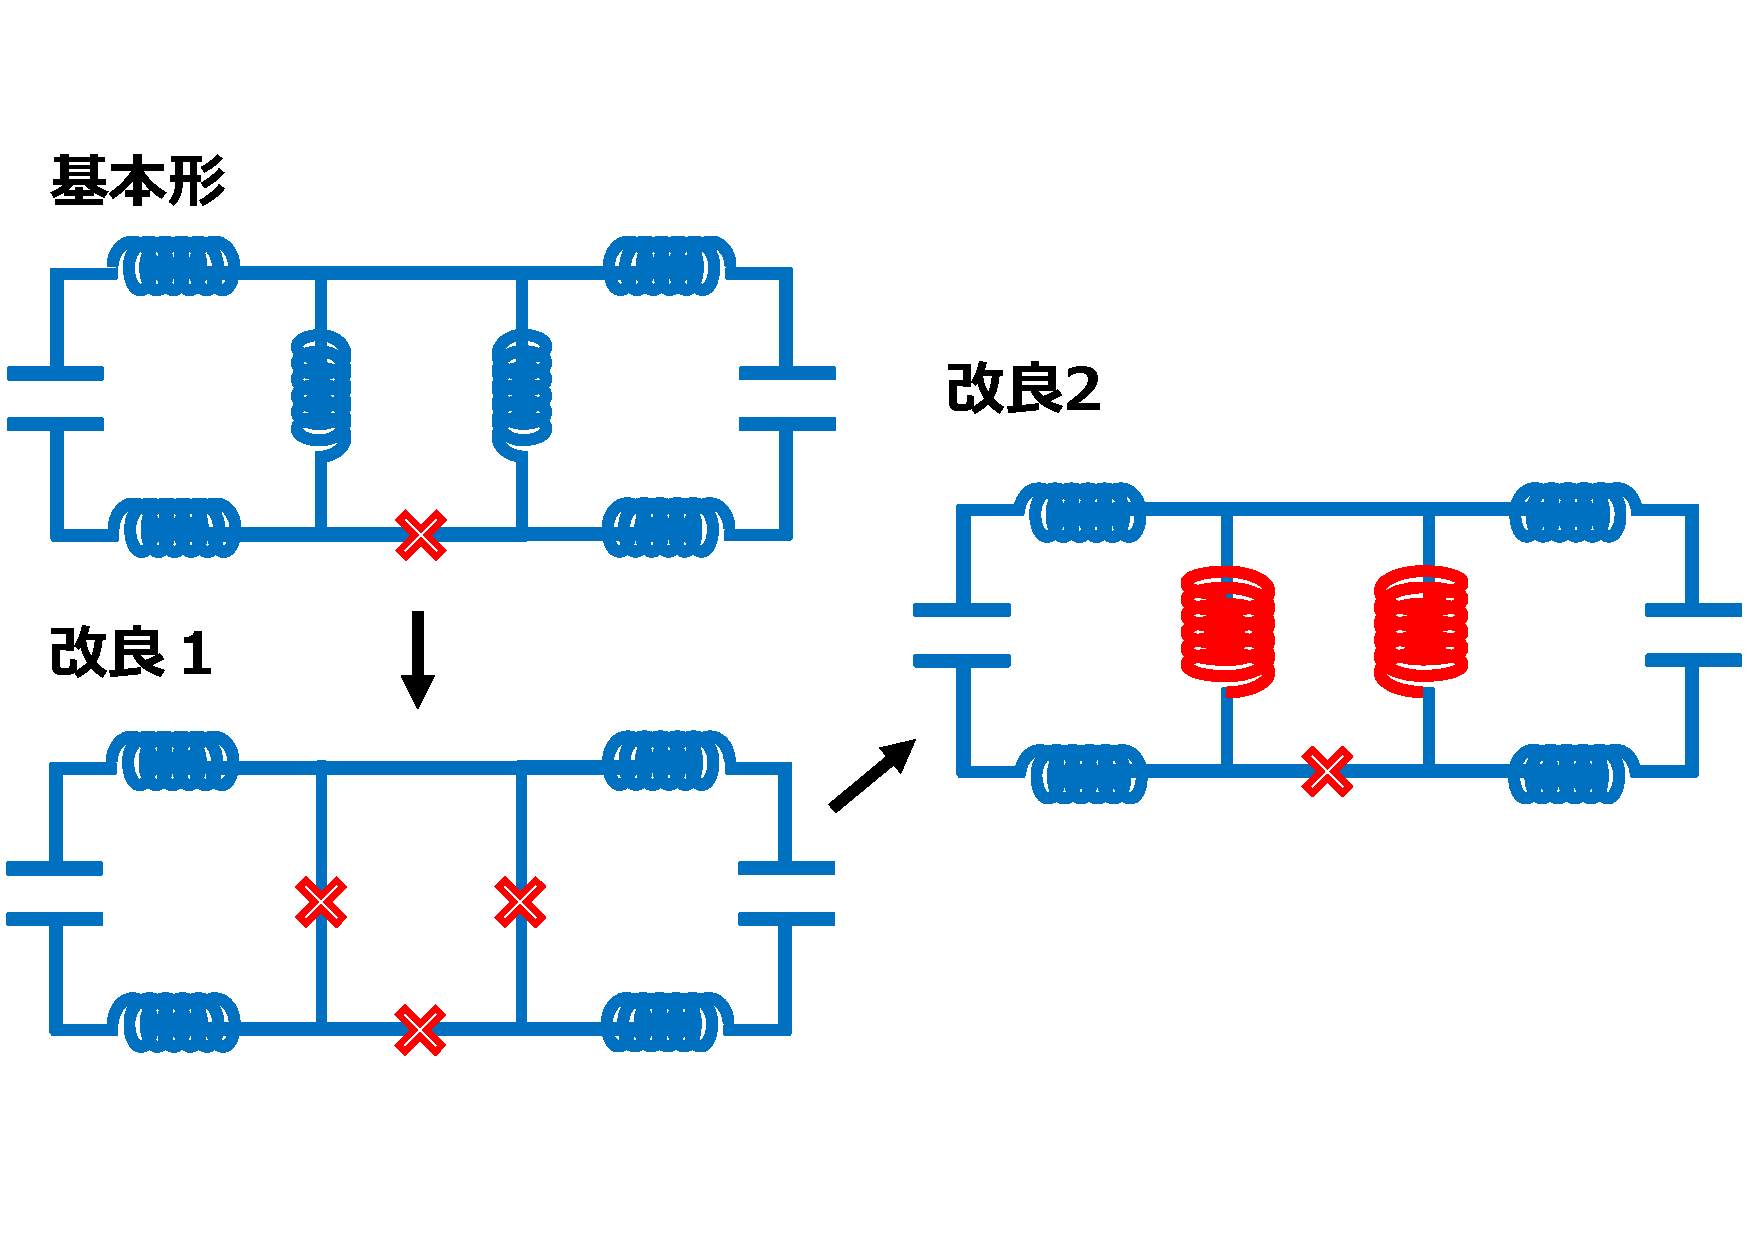
\includegraphics[width=14cm]{sample.pdf}
    %         \caption{サンプル図}
    %     \end{figure}
    %     上図は作成サンプルの回路図を模式的に表したものである。共振器とrf-SQUID間は線路に流れる電流により生じる磁場を介して結合している。模式図のように素子間が完全に接地した状態の結合のことをGalvanic結合と呼ぶ。この構造では、素子間の相互インダクタンスが接地部分の自己インダクタンスとほぼ等しくなるため非常に強力な相互インダクタンスを得ることができる。

    %     設計のポイントは①rf-SQUID-共振器間の相互インダクタンス増強と②rf-SQUIDスクリーニングパラメータの精密な製造である。この2つのパラメータは結合強度を向上する上で非常に重要な因子となる。
    %     この2つのパラメータが結合強度向上に大きく寄与するということを基本型であるrf-SQUIDの遷移スペクトルの計算を通して論拠する。
    % \subsection{遷移スペクトル計算}
    %     基本型の回路のハミルトニアンは
    %     \begin{equation}
    %         \hat{\mathcal{H}}=\hbar\left(\hat{a}^{\dagger }\ \hat{b}^{\dagger }\right)\left(\begin{array}{cc}
    %         \tilde{\omega}_{a} & g(\Phi ) \\
    %         g(\Phi ) & \hat{\omega}_{b}
    %         \end{array}\right)\left(\begin{array}{l}
    %         \hat{a} \\
    %         \hat{b}
    %         \end{array}\right)
    %     \end{equation}
    %     \begin{equation}
    %         = \hbar \hat{\omega}_{a} \hat{a}^{\dagger} \hat{a}+\hbar \hat{\omega}_{b} \hat{b}^{\dagger} \hat{b}+\hbar g(\Phi)\left(\hat{a}^{\dagger}\hat{b}+\hat{a} \vec{b}^{+}\right)
    %     \end{equation}

    %     である。式の前項2つが左右各共振器の調和振動子ポテンシャルである。最終項が結合項であり、この結合項に依存して2つの共振器が反発することを示す。各共振器の生成消滅演算子を
    %     \begin{equation}
    %         \hat{c}_{\pm}=\frac{\hat{a} \pm \hat{b}}{\sqrt{2}} \quad \hat{c}_{+}^{\dagger}=\frac{\hat{a}^{\dagger} \pm \hat{b}^{\dagger}}{\sqrt{2}}
    %     \end{equation}

    %     と置き換える。ここで演算子$\hat{c}_{\pm}$は各共振器の状態が混合した状態である。このように変換を行うと最終的に得られる状態は
    %     \begin{equation}
    %         \hat{H}=\hbar \Omega_+\hat{c}^{\dagger}_+\hat{c}_+ + \hbar \Omega_-\hat{c}^{\dagger}_-\hat{c}_- + \hbar \Delta\left(\hat{c}^{\dagger}_+ \hat{c}_- +\hat{c}^{\dagger}_- \hat{c}_{+}\right)
    %     \end{equation}

    %     \begin{equation}
    %         =\hbar\left(\begin{array}{cc}
    %         \hat{c}^{\dagger}_{+} & \hat{c}^{\dagger}_-
    %         \end{array}\right)\left(\begin{array}{cc}
    %         \Omega_{+} & \Delta \\
    %         \Delta & \Omega_{-}
    %         \end{array}\right)\left(\begin{array}{l}
    %         \hat{c}_{+} \\
    %         \hat{c}_{-}
    %         \end{array}\right)
    %     \end{equation}

    %     となる。この時$\Omega_+ = (\omega_a+\omega_b)/2 + g$、$\Omega_- = (\omega_a+\omega_b)/2 - g$、$\Delta = (\omega_a-\omega_b)/2$である。これより、2つの独立な調和振動子系は結合項$g$によって新たな基準モードで書き表すことができる。この新たな基底同士は元々の共振周波数の離調$(\omega_a-\omega_b)/2$で書き表すことができる。また変換前の基底、つまり左右の調和振動系の結合項$g$は新基底において新固有値の差分に現れる。これを図示すると以下のようになる。
    %     \begin{figure}[H]
    %         \centering
    %         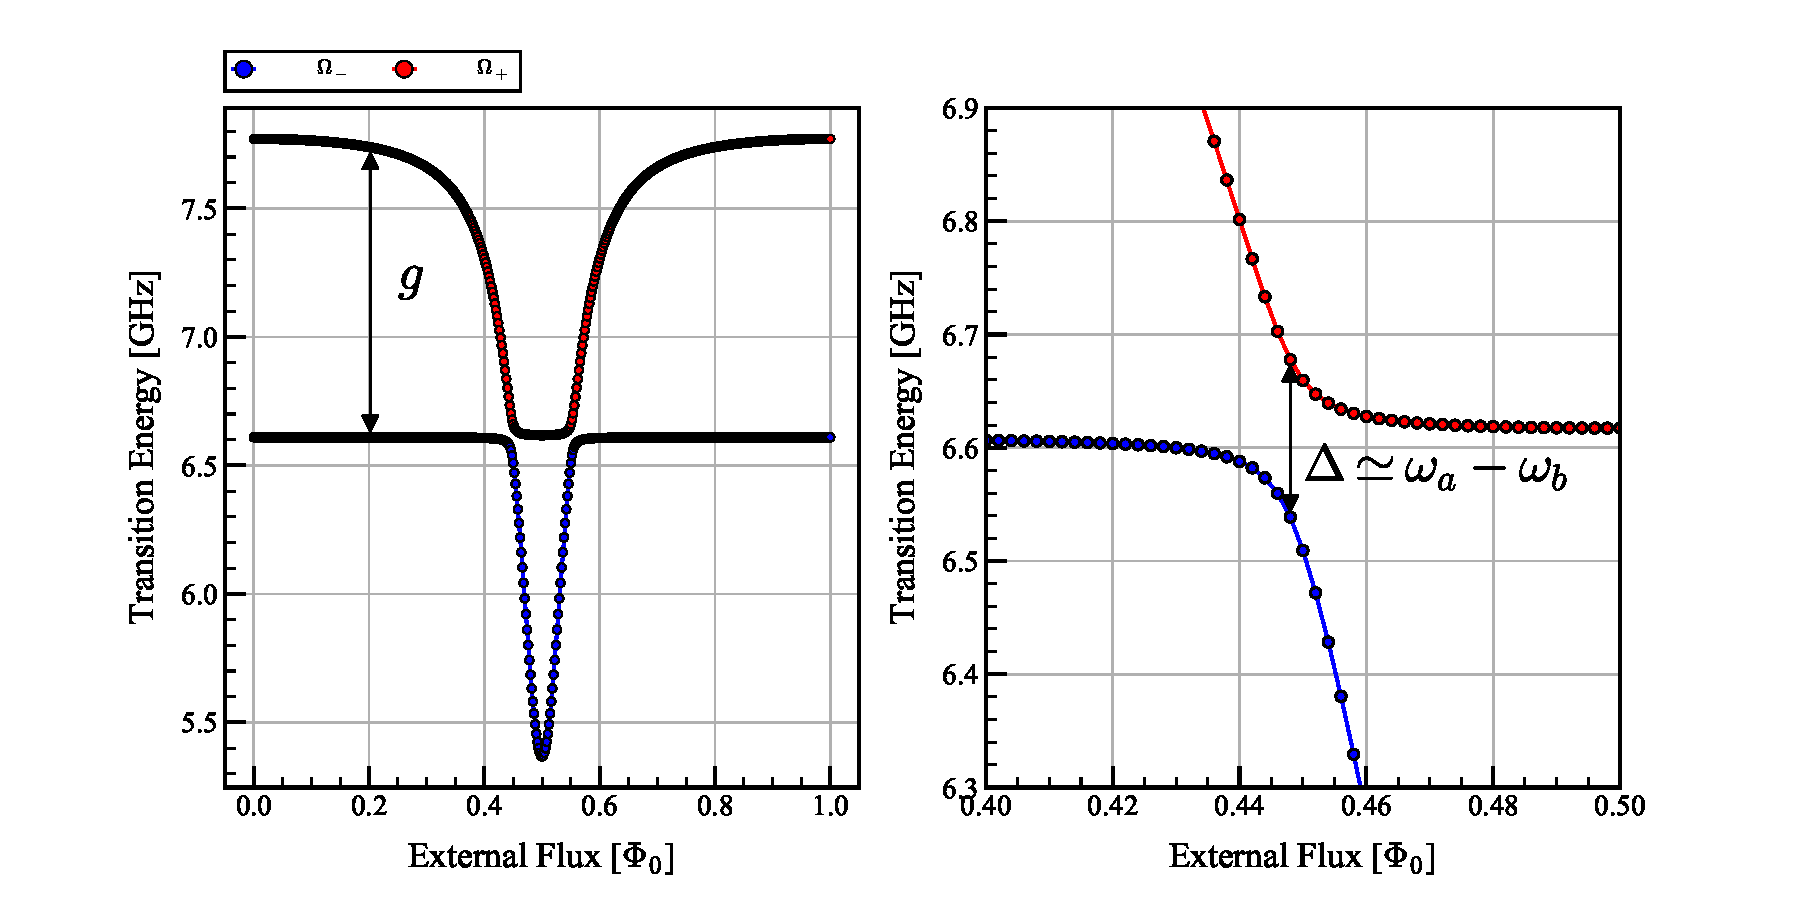
\includegraphics[width=16cm]{standard_eigen.pdf}
    %         \caption{遷移周波数図}
    %     \end{figure}
    %     つまり、測定において得られた2つの基準モードの差分を計算することにより元のハミルトニアンの結合強度gを見積もることができる。以下に上図に対応する外部磁束に対応する結合強度の図をプロットする。
    %     \begin{figure}[H]
    %         \centering
    %         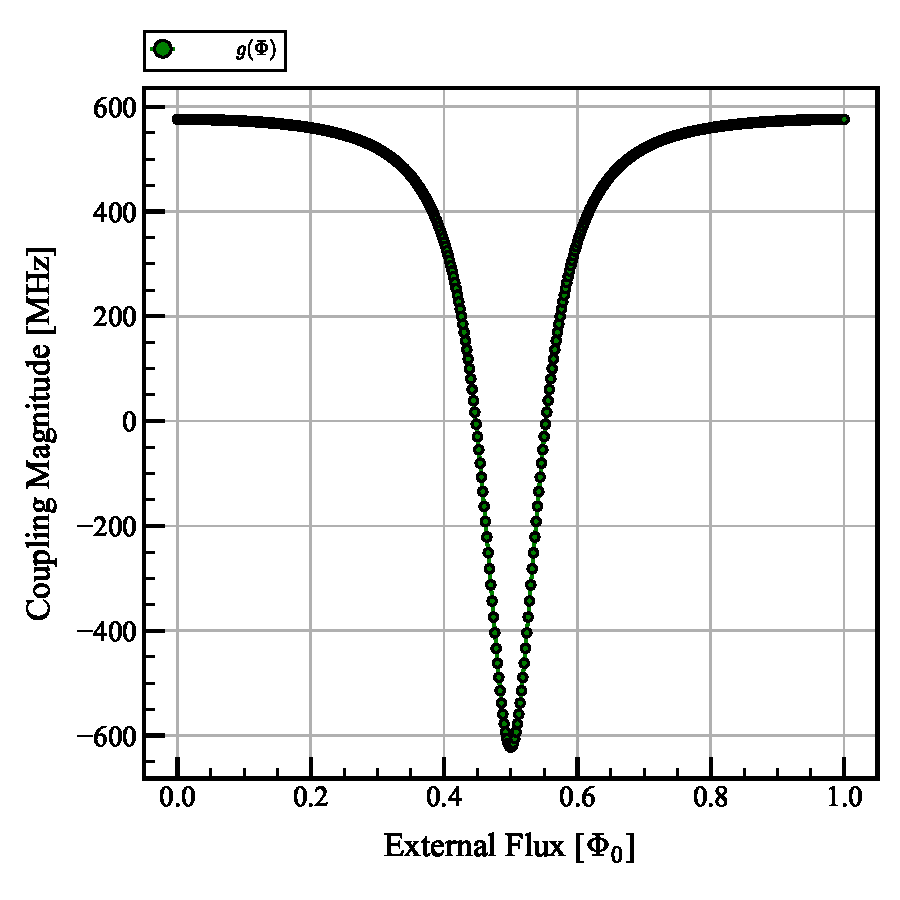
\includegraphics[width=7cm]{standard_coupling.pdf}
    %         \caption{結合強度図}
    %     \end{figure}

        % 既に述べたように今回作成した結合回路において強度をドメスティックに変えるパラメータはrf-SQUIDのスクリーニングパラメータとrf-SQUIDと共振器間の相互インダクタンスである。それぞれのパラメータを変えた時にどのように結合強度が変化するのを示した図が以下である。

        % また、外部磁束を0.5に固定子、$\beta$の値のみを変更することによる結合強度の対応をプロットすると$\beta$が0.8を超えたあたりで急激に結合強度が変化していることがわかる。
        % % \begin{figure}[H]
        % %     \centering
        % %     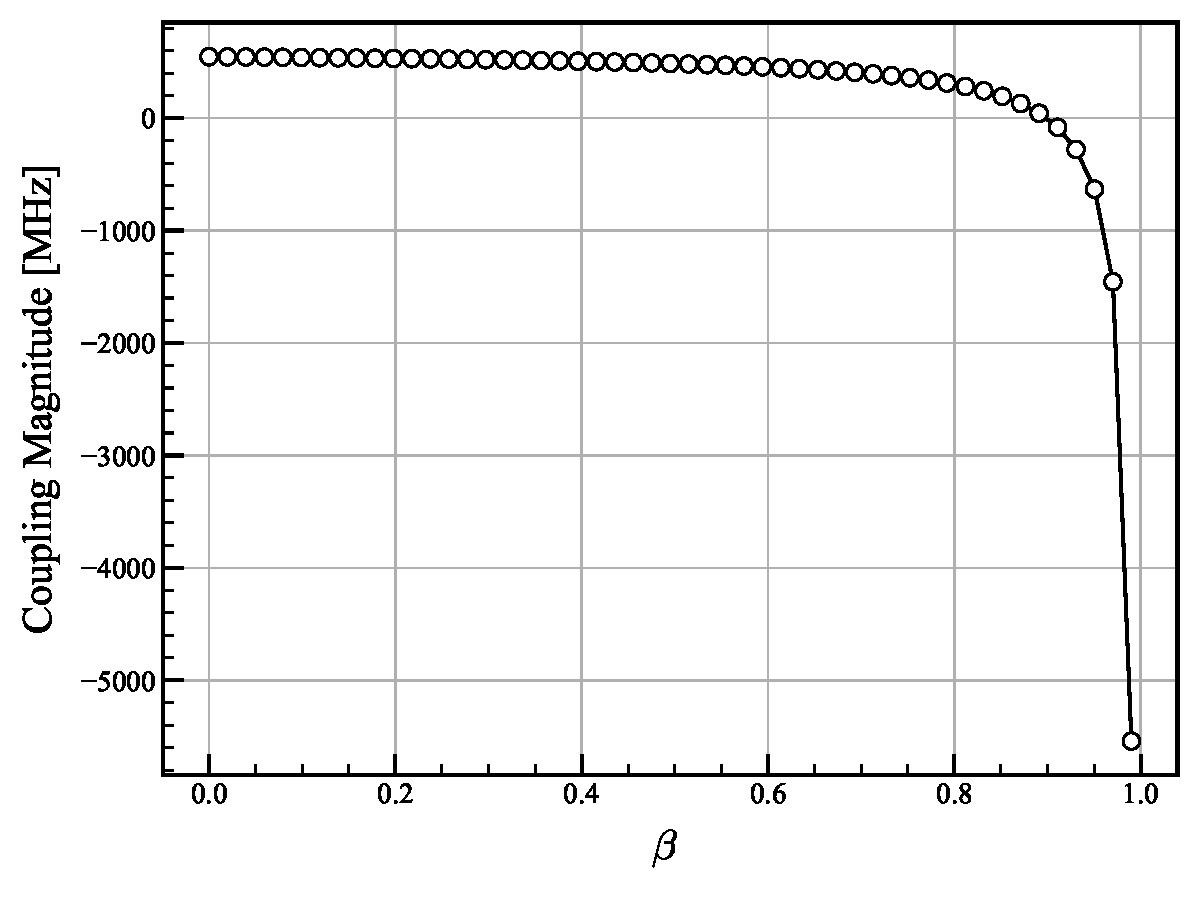
\includegraphics[width=8.5cm]{standard_coupling_betasweep.pdf}
        % %     \caption{結合強度の$\beta$依存性}
        % % \end{figure}
        % スクリーニングパラメータが1を超えるとこの関数は発散してしまうため、最適な動作点としては$0.8<\beta<0.95$付近が妥当であると考えられる。しかしながら、後述するが実際にはスクリーニングパラメータをこの領域内に収めることは非常に困難である。
        % スクリーニングパラメータはジョセフソンインダクタンス$Lj$とrf-SQUIDのループインダクタンスLsにより$\beta=Ls/Lj$と表現されるが仮にLsの値を0.224[nH]で設計した場合
        % \begin{equation*}
        %     L_{jdes} = 0.258 \pm 0.022\ [nH]
        % \end{equation*}
        % 経験的にジョセフソン接合の作成にはインダクタンスにしてOOnHのばらつきが出るため、再現性が非常に低くなる。

        \begin{figure}[H]
            \centering
            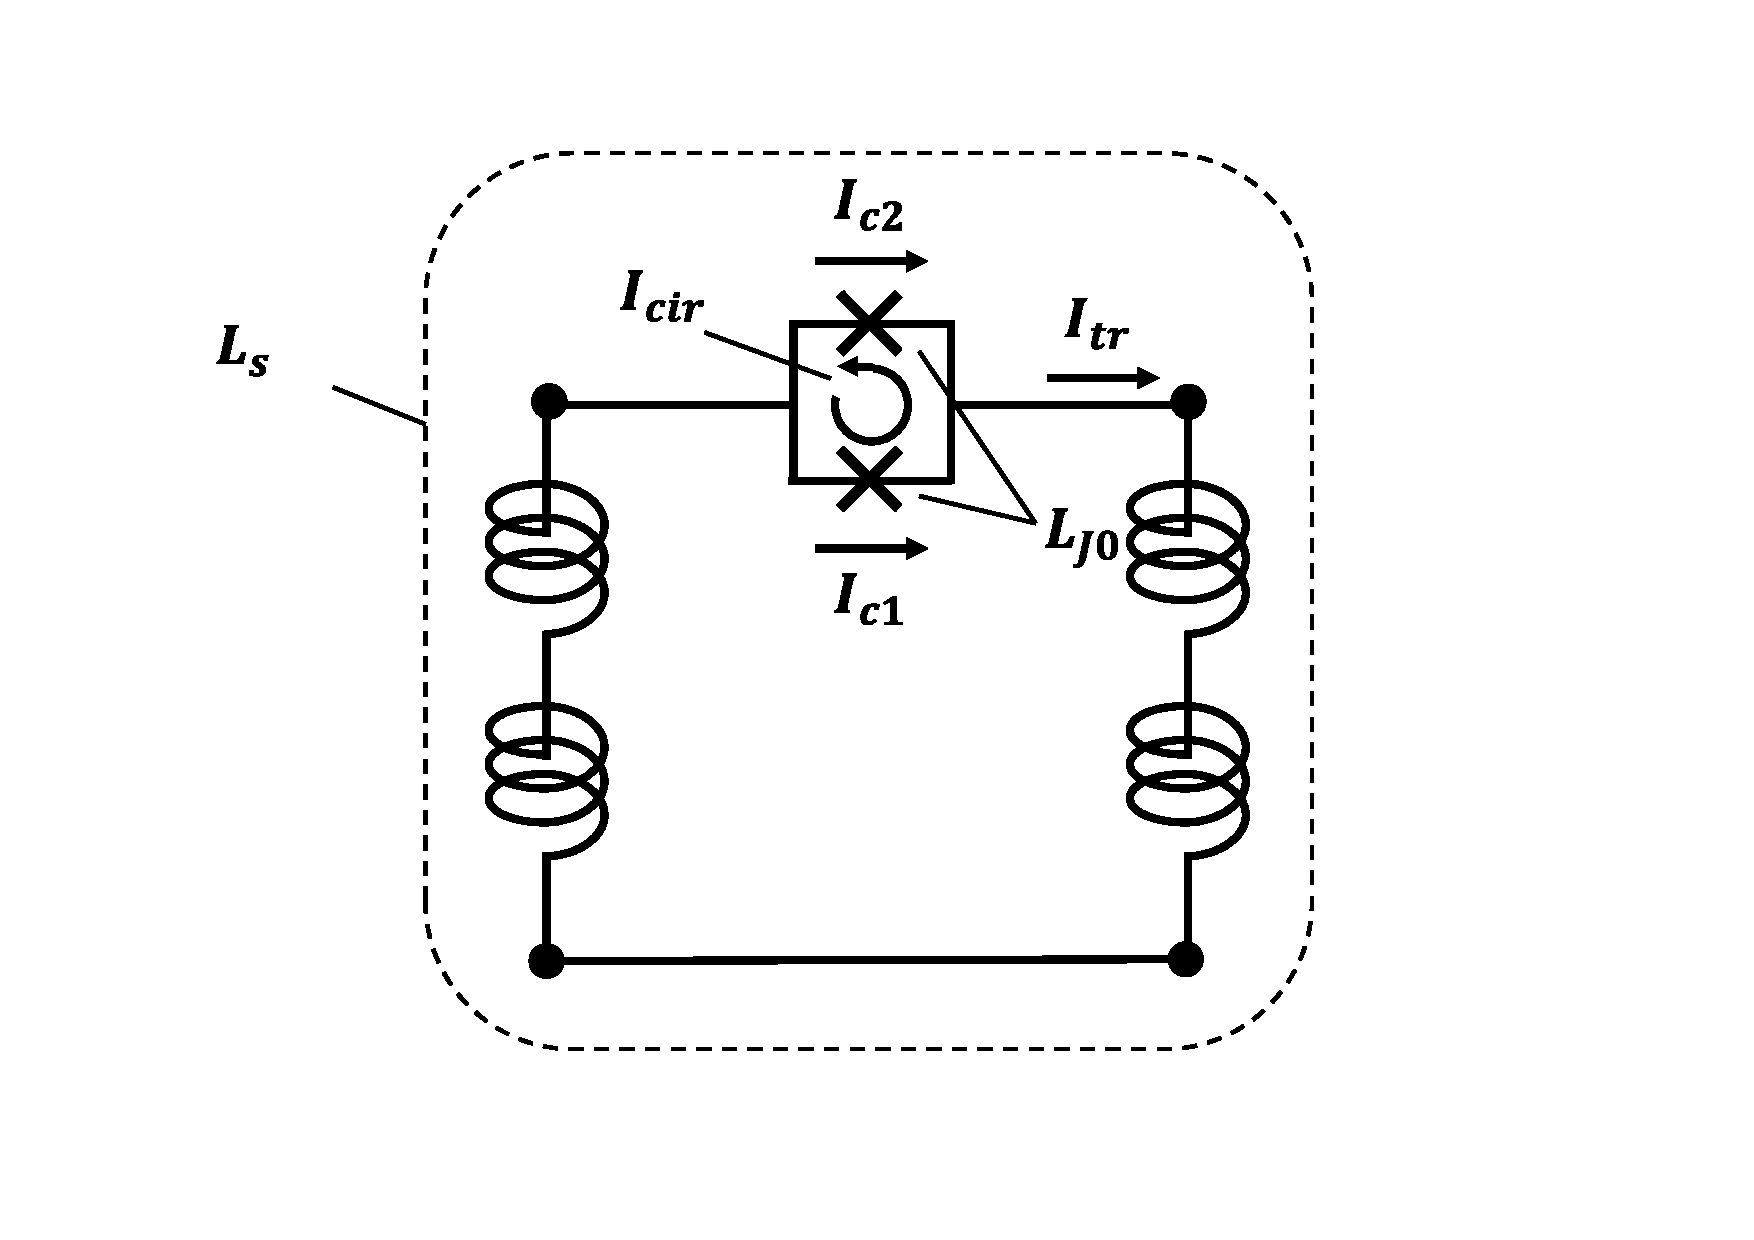
\includegraphics[width=12cm]{dc-squid_circuit.pdf}
            \caption{dc-SQUIDの回路図}
        \end{figure}
        dc-SQUIDを流れる電流$I_{tr}$は2つの電流$I_{c1},I_{c2}$により
        \begin{equation}
            I_{tr} = I_{c1} + I_{c2}
        \end{equation}
        と書き表せる。また、超伝導ループを周回する電流を$I_{cir}$とすると2つの電流は
        \begin{subequations}
            {\jot=10pt
        \begin{eqnarray}
            I_{c1}  = I_{tr}/2+I_{cir}\\
            I_{c2}  = I_{tr}/2-I_{cir}
        \end{eqnarray}
        }
        \end{subequations}
        である。ジョセフソン接合の位相差をそれぞれ$\phi_1,\phi_2$とすると臨界電流$I_c$において
        \begin{subequations}
            {\jot=10pt
        \begin{eqnarray}
            I_{c1}  = I_{c}sin(\phi_1)\\
            I_{c2}  = I_{c}sin(\phi_2)
        \end{eqnarray}
        }
        \end{subequations}
        とも表記できる。超伝導ループの周期条件より位相差$\phi_2-\phi_1$について$2\pi$の整数倍が要請され
        \begin{equation}
            \phi_{2}-\phi_{1}=\frac{2 \pi}{\Phi_{0}} \Phi_{\mathrm{dc}}=\frac{2 \pi}{\Phi_{0}}\left(\Phi_{\mathrm{ext}}+L_{dc} I_{cir}\right)
        \end{equation}
        ここで$\Phi_{dc}$はdc-SQUIDを貫く磁束の総和であり、外部磁場$\Phi_{ext}$とループが持つ自己インダクタンスによる遮蔽磁場$\L_{dc}I_{cir}$の和である。dc-SQUIDのスクリーニングパラメータが
        \begin{equation}
            \beta_{dc}:=\frac{2 L I_{c}}{\Phi_{0}} \ll 1
        \end{equation}
        であることを仮定すると、ループを周回する電流とジョセフソン接合の臨界電流は$I_{cir}<I_{c}$であるため、ループを貫く磁場は実質$\Phi_{dc} = \Phi_{ext}$であると考えてよい。すなわち
        \begin{equation}
            I=I_{c}\left[\sin \phi_{1}+\sin \left(2 \pi \frac{\Phi_{\text {ext }}}{\Phi_{0}}+\phi_{1}\right)\right]
        \end{equation}
        ここで
        \begin{equation}
            \chi:=\phi_{1}+\pi \frac{\Phi_{\text {ext }}}{\Phi_{0}}
        \end{equation}
        と置くことで三角関数の加法定理より
        \begin{equation}
            I=2 I_{c} \cdot \sin \chi \cdot \cos \left(\pi \frac{\Phi_{\mathrm{ext}}}{\Phi_{0}}\right)
            \end{equation}
        が導かれる。$\sin\chi$は-1から1の範囲で変動するため、dc-SQUIDを流れる電流の最大値は
        \begin{equation}
            I_{s, \max }=2 I_{c}\left|\cos \left(\pi \frac{\Phi_{\text {ext }}}{\Phi_{0}}\right)\right|
        \end{equation}
        と求まる。よってdc-SQUIDは外部磁場によって変調可能なジョセフソンインダクタンス
        \begin{equation}
            L_{\mathrm{dcSQUID}}\left(\Phi_{\mathrm{ext}}\right)=\frac{\hbar}{2 e I_{s, \max }}=\frac{\Phi_{0}}{4 \pi I_{c}\left|\cos \left(\pi \frac{\Phi_{a}}{\Phi_{0}}\right)\right|}
        \end{equation}
        として扱うことが可能になる。
        rf-SQUID中の単一ジョセフソン接合をdc-SQUIDに置き換えることにより新たにスクリーニングパラメータ$\beta_{eff}$を定義し直すと
        \begin{equation}
            \beta_{eff}(\Phi_{ext}) = \frac{4\pi L_{s}I_{c}\left|\cos \left(\pi \frac{\Phi_{a}}{\Phi_{0}}\right)\right|}{\Phi_0}=\frac{2L_s\left|\cos \left(\pi \frac{\Phi_{a}}{\Phi_{0}}\right)\right|}{L_{J0}}
        \end{equation}
        以下に外部磁束に対するスクリーニングパラメータの応答を示す。
        \begin{figure}[H]
            \centering
            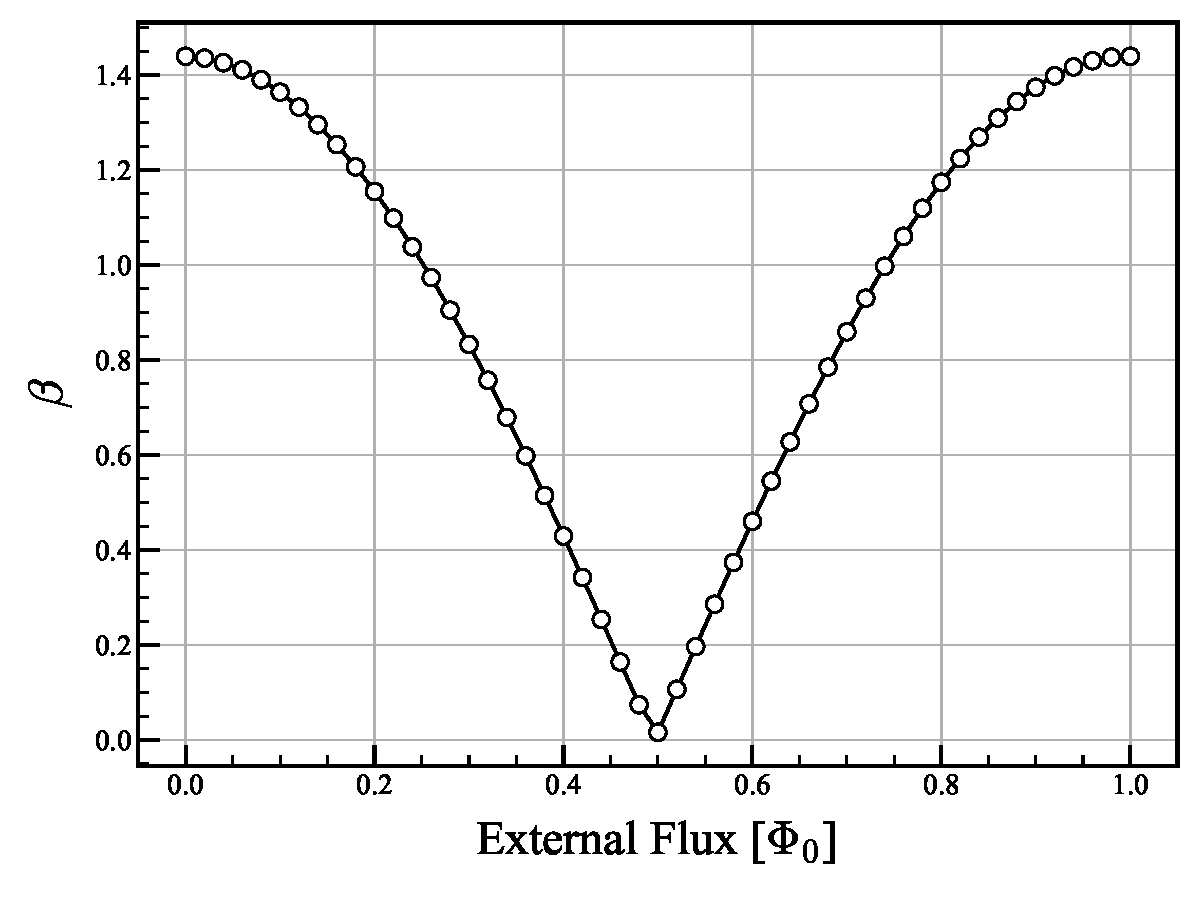
\includegraphics[width=8cm]{dc-squid.pdf}
            \caption{dc-SQUIDによる$\beta$変調}
        \end{figure}
        % この素子によりrf-SQUIDのジョセフソンインダクタンスを外部磁束によって変調することが可能となった。
        % 次にrf-SQUIDと共振器間の相互インダクタンスを向上させる手法について考える。
        % 今回採用した方法はミアンダインダクタンスを用いたものである。ミアンダインダクタンスは細線を蛇行させることにより各線路の相互インダクタンス、単純な線路長の増加によりインダクタンスを線路エリアに対して大きくすることができる。この設計において相互インダクタンスに注目することとなった経緯を説明する。
        % 修士の研究において大別して3種類のデバイスを測定したと述べたがこのうちJLCCの結果を受けてである。このサンプルはジョセフソン接合をrf-SQUIDと共振器間に挿入することで、ジョセフソンインダクタンスを用いて相互インダクタンスを強める目的で導入した。結果として望むような成果は得られなかったが次の2つの収穫が得られた。

        % ①正方向の結合強度を向上する手段として相互インダクタンスの寄与は非常に大きいこと。
        
        % ②相互インダクタンスはその大きさの2乗によって結合強度を増強すること。
        
        % スクリーニングパラメータ$\beta$の精密な操作が結合強度を急激に増加させることは既に述べたが、結合素子として扱う際には磁束の急激な変化は望ましくない。操作が困難になることはもちろん急激な値の変化は解析をするさいにも困難を要する。そこで、まずは相互インダクタンスで可能な限りな結合強度の増強を試みる。
        % また、共振器間の1次結合(直接的な相互インダクタンスを強めるためにrf-SQUIDの構造も縦長なループ構造へと修正した。
        % \begin{figure}[H]
        %     \centering
        %     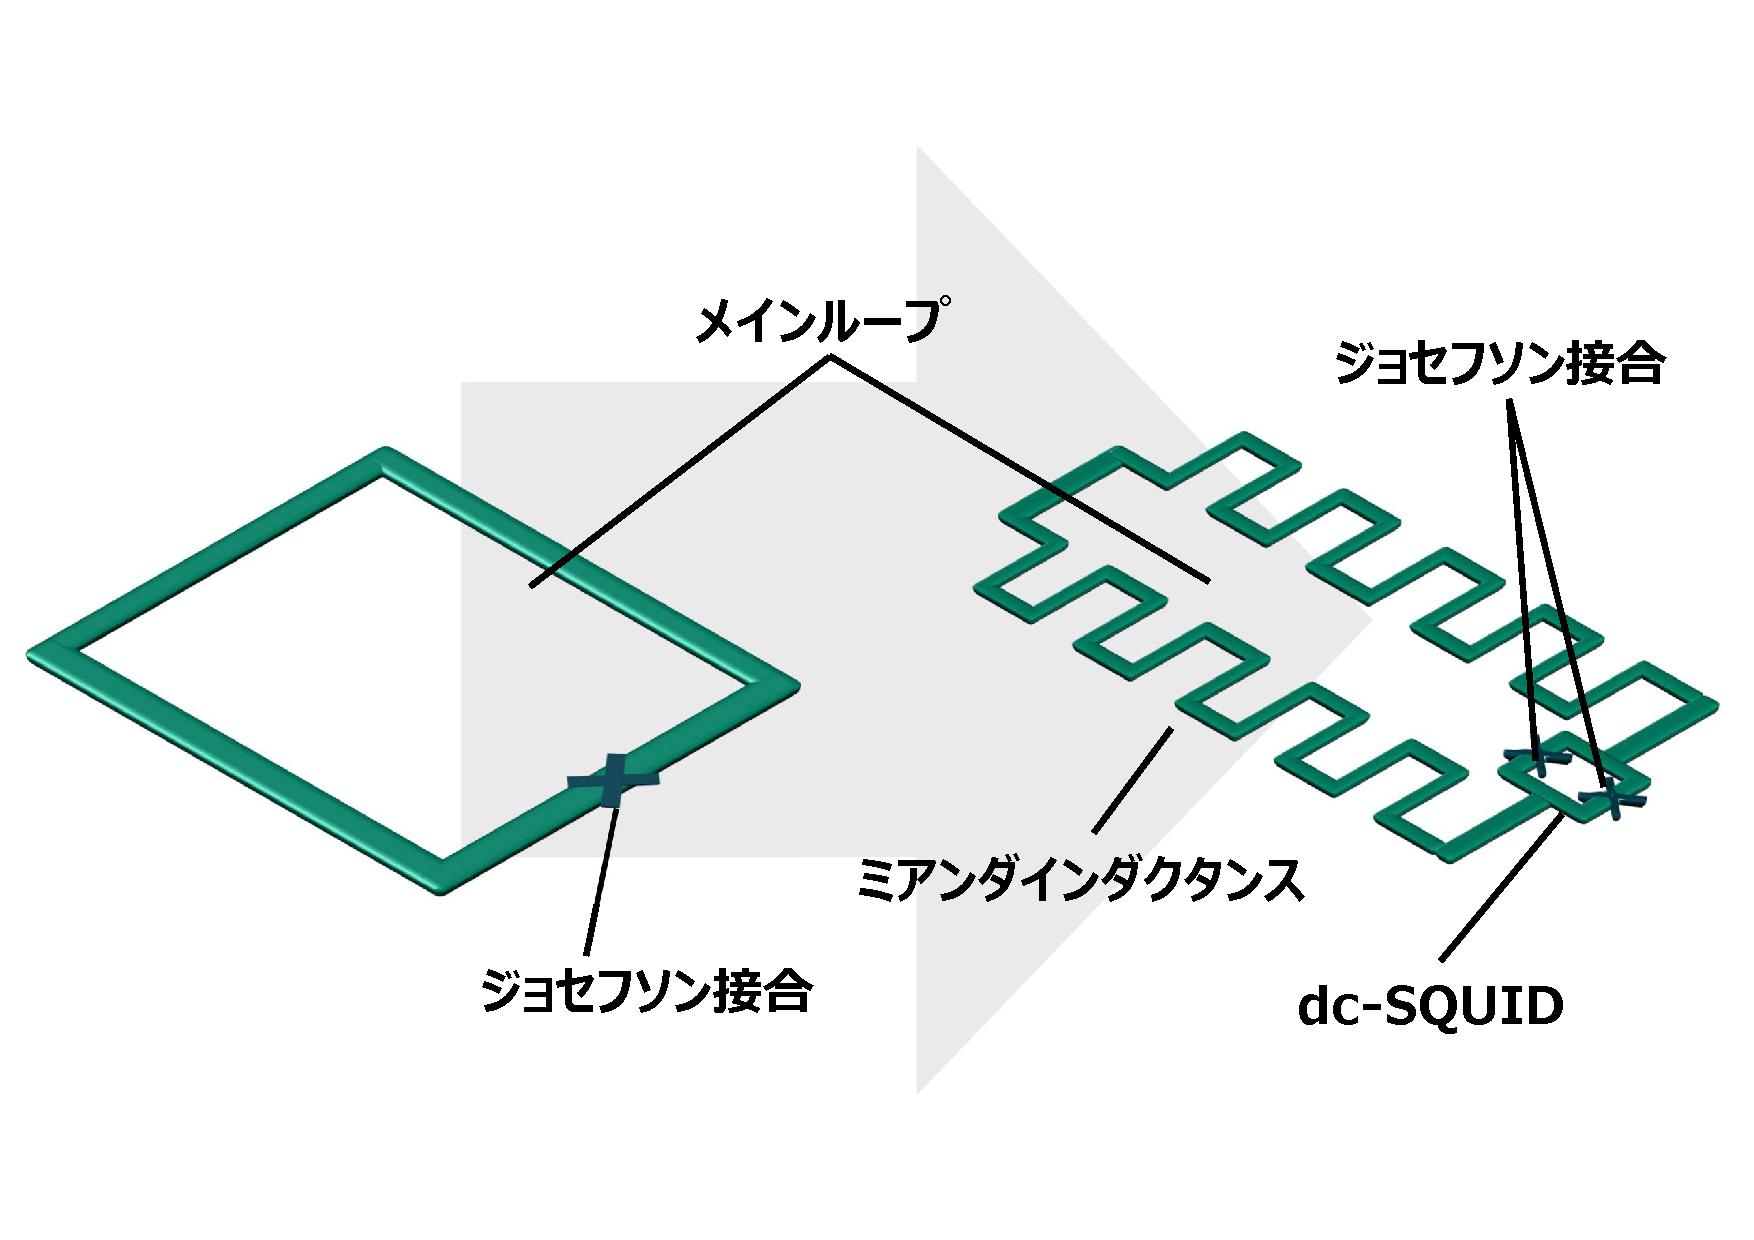
\includegraphics[width=12cm]{samplefigure.pdf}
        %     \caption{aMLCCの模式図}
        % \end{figure}
        % 次に配線構造を考える。サンプル上に載せる配線の本数は少なければ少ないほどに良い。特に磁束バイアスを用いる場合、クロストークを考慮する必要がある。今回のサンプルでは少なくとも2つの独立な電流源が必要となる。1つはdc-SQUIDにバイアスしてスクリーニングパラメータを調整する電流源、もう一つがrf-SQUIDのメインループを貫き、結合素子の強度を変更するための磁束バイアスである。ここでは配線構造について考える。
        % 実験環境ではサンプル上に載せるオンチップバイアスラインとサンプルをマウントするサンプルホルダー上に積載しているグローバルフラックスを用いることができる。配線本数を減らすという観点ではこのグローバルフラックスを利用するのが好ましい。しかしながら、グローバルフラックスはサンプル全体に均一な磁場がかかるため、メインループとdc-SQUIDのループ面積比を極端に差別化することで独立な操作がしやすいように工夫した。
        % \begin{figure}[H]
        %     \centering
        %     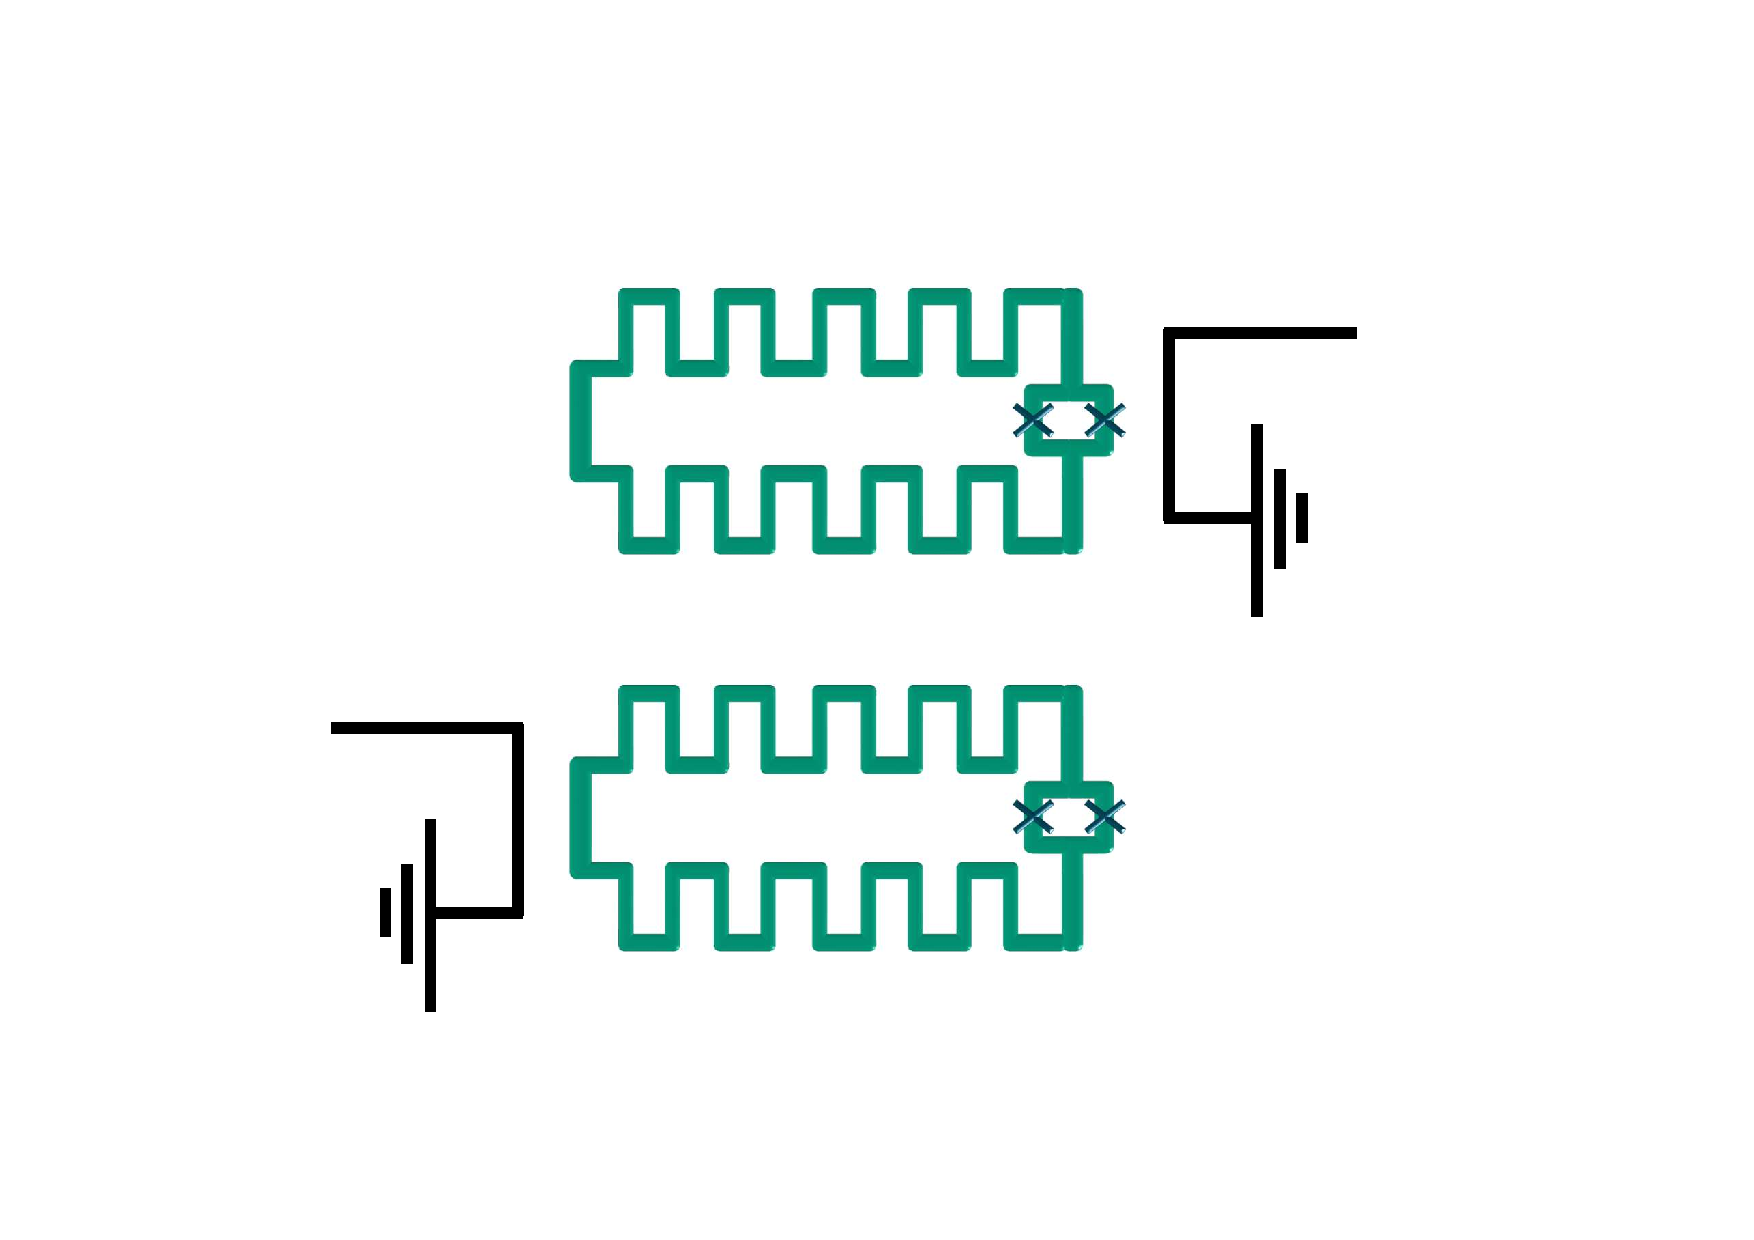
\includegraphics[width=10cm]{配線.pdf}
        %     \caption{aMLCCの模式図}
        % \end{figure}
        % 一方をグローバルフラックスで駆動し、もう一方をオンチップバイアスで駆動することを考える場合、配線の仕方は上記図のような2つの方法が考えられる。今回はメインループ側にオンチップバイアスを取り付けた。グローバルバイアスを全体に印加しているためメインループ、dc-SQUIDを均一磁場が貫く。貫く磁束量子の本数はループの面積比に依存するため、メインループの面積比をdc-SQUIDの100倍にすることで差別化した。まずは上部の配線構造について説明を加えるとこの配線構造ではグローバルバイアスでrf-SQUIDを貫く磁束を固定した上で新たにオンチップバイアスでdc-SQUIDに磁束を印加することでrf-SQUIDのスクリーニングパラメータを調整することができる。この配線構造で問題となるのはオンチップバイアスラインとrf-SQUIDのメインループが非常に近接しているということである。クロストークを可能な限り抑制することを考えるとこの配線は望ましくない。
        % 次に下部の配線構造であるが、この場合ではグローババイアスでdc-SQUIDを貫く磁束を固定した上でrf-SQUIDを貫く磁束をオンチップバイアスで調節することを目的としている。この場合オンチップバイアスがdc-SQUIDに影響するクロストークは非常に小さいといえる。ループの形状を縦長にするという工夫はクロストークを抑制するという点でも非常に合理的であることがわかる。しかし、クロストークがいかに小さいとはいえ、オンチップバイアスからdc-SQUIDに寄与するクロストークは少なからず存在する。測定を行う際にはそれぞれの電流源がそれぞれのループに寄与するクロストークをインダクタンス行列を用いて評価する。

    \subsection{共振器}
        共振器には超伝導準集中定数素子を用いた。超伝導量子回路で一般的に使用されているCPW型共振器はグランドと伝送線路の距離を伝送損失の少ない50$\Omega$で保つことで単位長さあたりのキャパシタンス$Cp.u.l$とインダクタンス$Lp.u.l.$を求め、伝送線路の長さを乗じることで回路全体のキャパシタンスとインダクタンスを決定している。非常にこの構造は伝送損失が少なく非常に簡便に共振器の設計ができる点がメリットとなる。他方で単位長さあたりのキャパシタンスとインダクタンスが一定にするため複雑な構造をつ繰り出すことはできない。また集中定数回路のように局所的に共振パラメータを調節することには向かないといえる。他方で今回採用した準集中定数型の共振器は意図的に局所的なキャパシタンスとインダクタンスを設けることでLC共振器をつくり出している。この場合共振周波数は回路の局所的な共振パラメータにより求まり、線路長には依らない。
        共振器のパラメータ計算には手計算に依る解析的な方法と電磁界シミュレーションに依る2つの方法を用いた。電磁界シミュレーションにはAWR社のマイクロウェーブオフィス(ver14.03)を使用した。
    \subsection{電磁界シミュレーション}
        共振器の1次結合は電磁界シミュレータ―を用いて算出した。シミュレーションした構造は以下の2つである。
        \begin{figure}[H]
            \subfigure{
            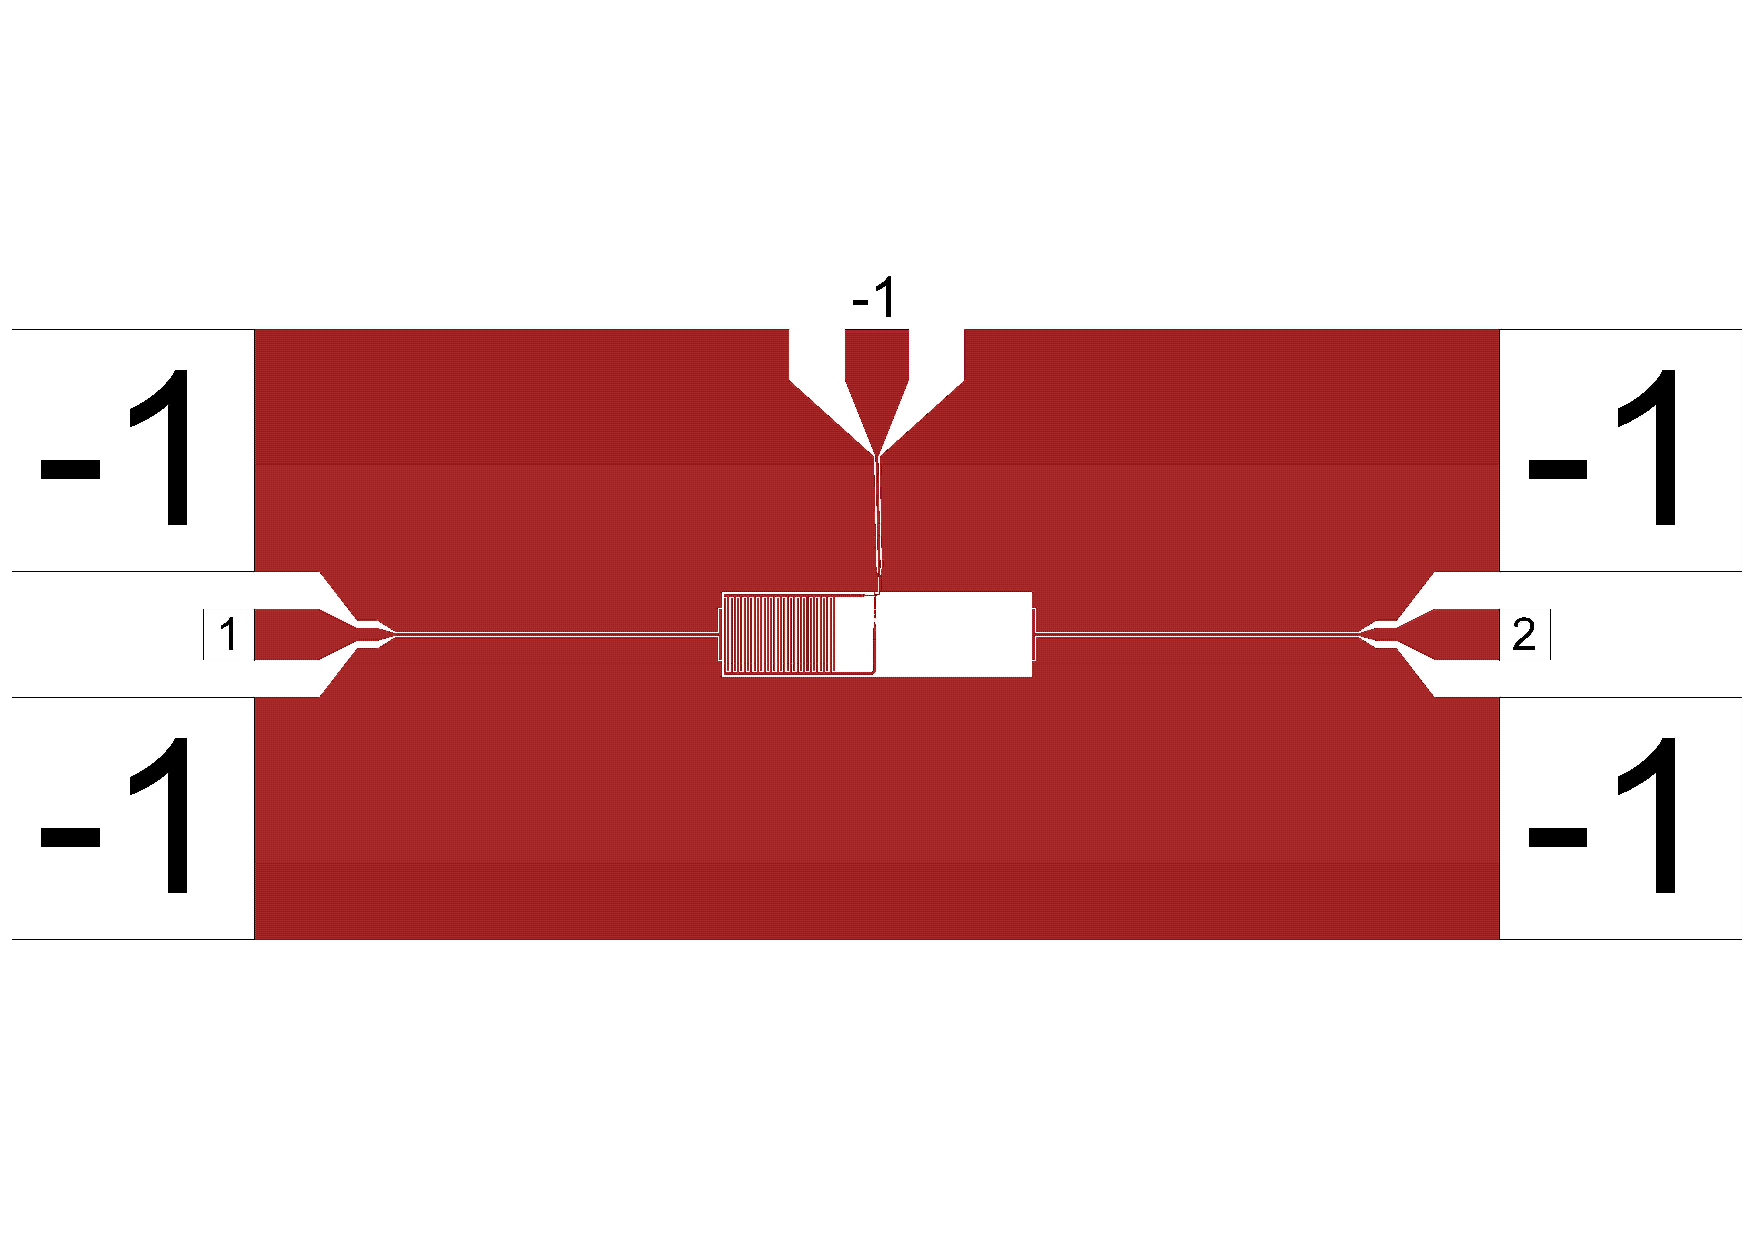
\includegraphics[width=0.5\columnwidth]{resonator_design_for_mwo.pdf}
            }
            \subfigure{
            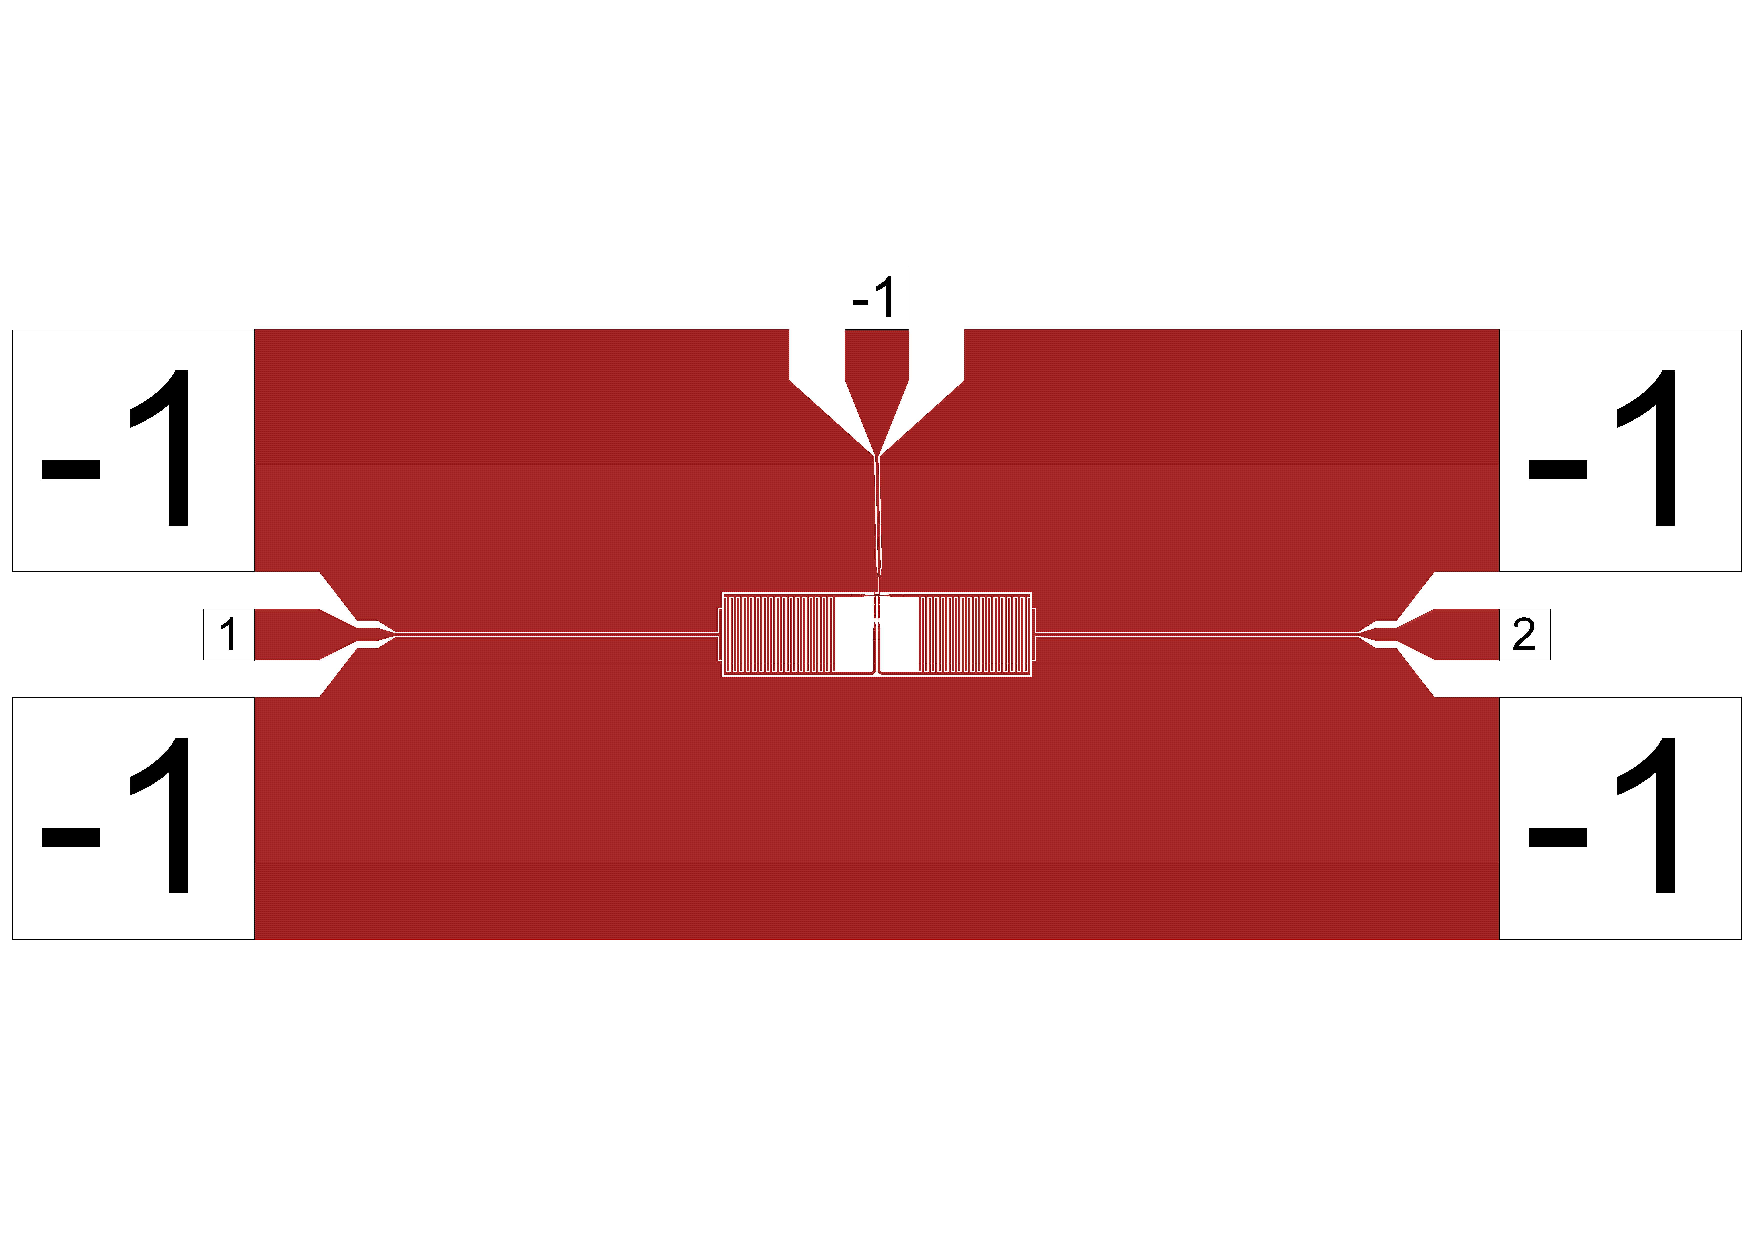
\includegraphics[width=0.5\columnwidth]{coupled_resonator_mwo.pdf}
            }
            \caption{電磁界シミュレーションに使用した構造}
        \end{figure}
        また、電磁界シミュレーションでは電流分布も表示することが可能である。
        図中右側の構造は左の構造を左右対象に配置したものである。すなわち共振周波数は左右の共振器で同一になっている。この構造を電磁界シミュレーションすると図中左の構造物をBare Resonaotr図中右側の構造物を左からResonator A、Resonator Bと表現する。Resonator AとResonator BはBare Resonatorを中点としてそれぞれ結合強度の1/2で反発することが予想される。このシミュレーションによってもっと待った共振周波数の差は共振器間の1次結合gに対応する。
        \begin{figure}[H]
            \centering
            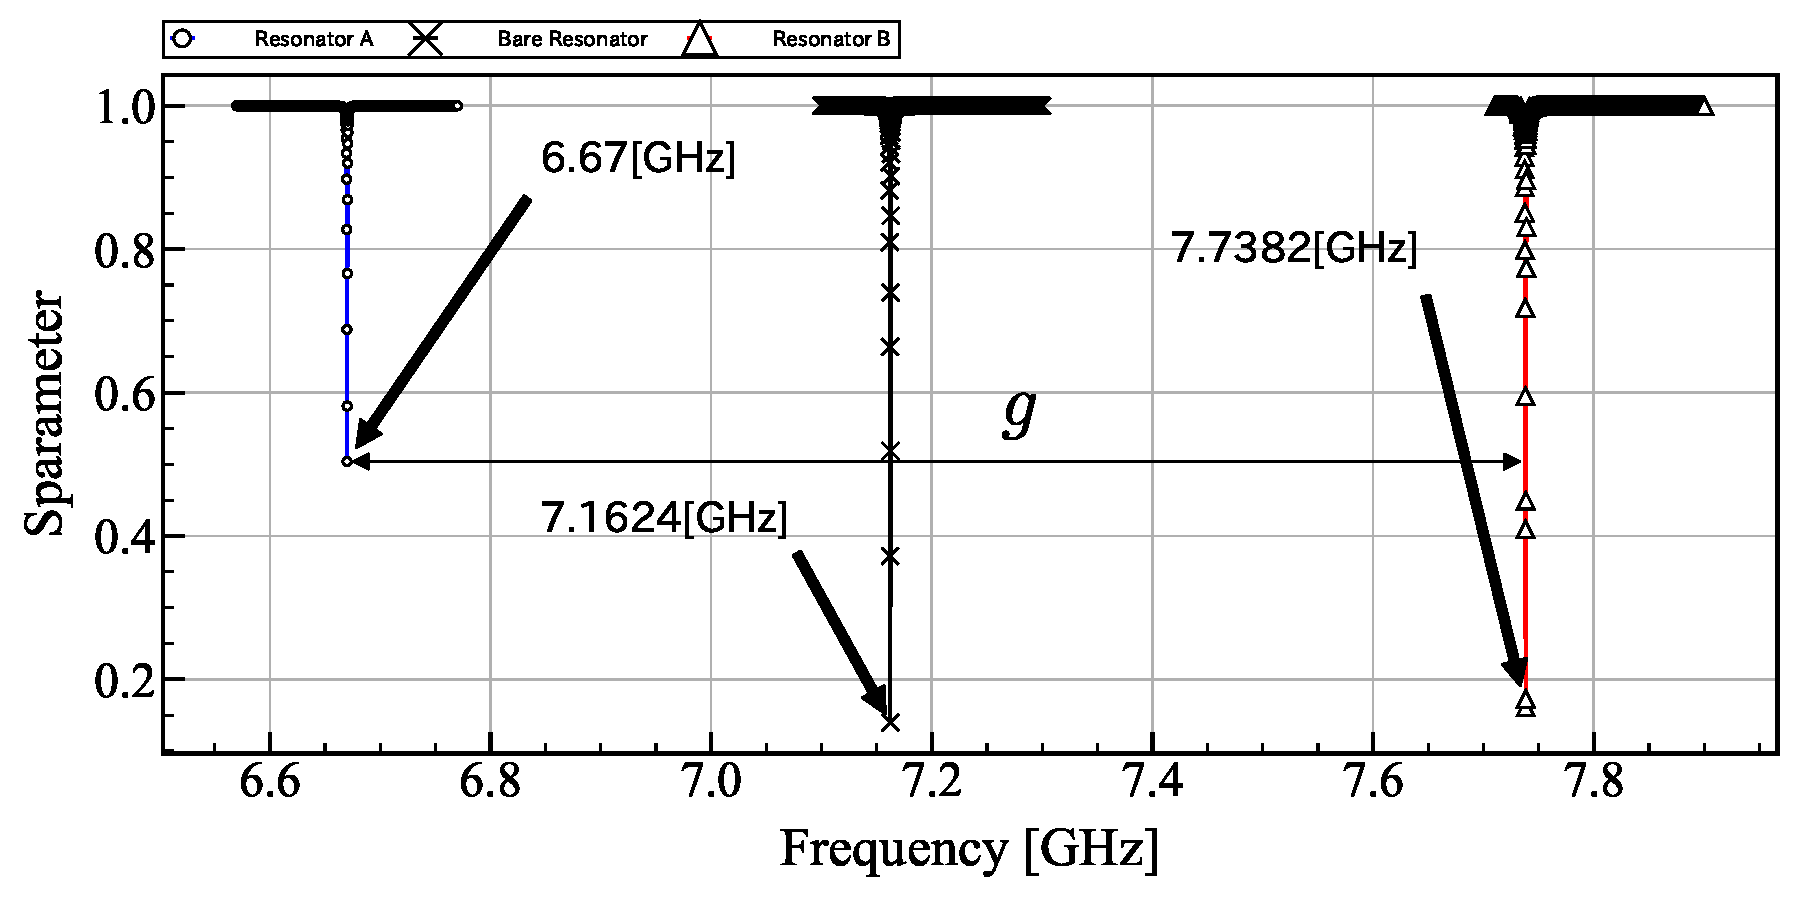
\includegraphics[width=12cm]{mwo.pdf}
            \caption{dc-SQUIDによる$\beta$変調}
        \end{figure}
        構造が同じ共振器間に結合強度gが存在する場合、共振器は結合強度に依存して反発する。これは電気回路からも求めることができる。補足に詳しい計算を記したので参考されたい。
        電磁界シミュレーションによって算出された共振周波数を以下に示す。
        \begin{table}[h]
            \caption{共振周波数}
            \centering
            \begin{tabular}{@{}cc@{}}
            \toprule
                           & Frequency [GHz] \\ 
                           \hline \hline
            Resonator A    & 6.6700          \\
            Resonaotor B   & 7.7382          \\
            Bare Resonator & 7.1624          \\ \bottomrule
            \end{tabular}
            \end{table}
        また、同時に各共振器に流れるゼロポイントフィールド電流$I_{ZPF}$は及び結合強度、相互インダクタンスについては
        \begin{table}[h]
            \caption{結合共振器のパラメータ}
            \centering
            \begin{tabular}{@{}cc@{}}
            \toprule
            Parameter & Value    \\ 
            \hline \hline
            Current        & 5.740 nA \\
            Mutual Inductance       & 0.107 nH \\ 
            coupling constant         & 534 MHz  \\\bottomrule
            
            \end{tabular}
            \end{table}
        次に電磁界シミュレータ―を用いてBare Resonatorのインダクタンスとキャパシタンスを求める。
        図OOについて低周波でのアドミッタンスを求める。低周波、直流源に対してはキャパシタンスがインピーダンスとして強く現れる。この特性を用いてBare Resonatorに置けるキャパシタンスとインダクタンス、特にミアンダインダクタンスの評価をする。
        ミアンダインダクタンスを評価する上で上記のデザインに加えて新たに以下のようなデザインについてもシミュレーションを行った。
        \begin{figure}[H]
            \centering
            \includegraphics[width=12cm]{bareresonator_zoom.pdf}
            \caption{dc-SQUIDによる$\beta$変調}
        \end{figure}
        この共振器デザインにはミアンダインダクタンスが含まれていない。その他の構造物(キャパシタンス)は同一のものを使用しておりこの2つの構造物の差はほぼミアンダインダクタンスの可否に依存する。そこで上記の方法でキャパシタンスをそれぞれ求め、回路全体のインダクタンスの差分をとることでミアンダインダクタンスの値を求めた。結果は以下である。
        \begin{figure}[H]
            \centering
            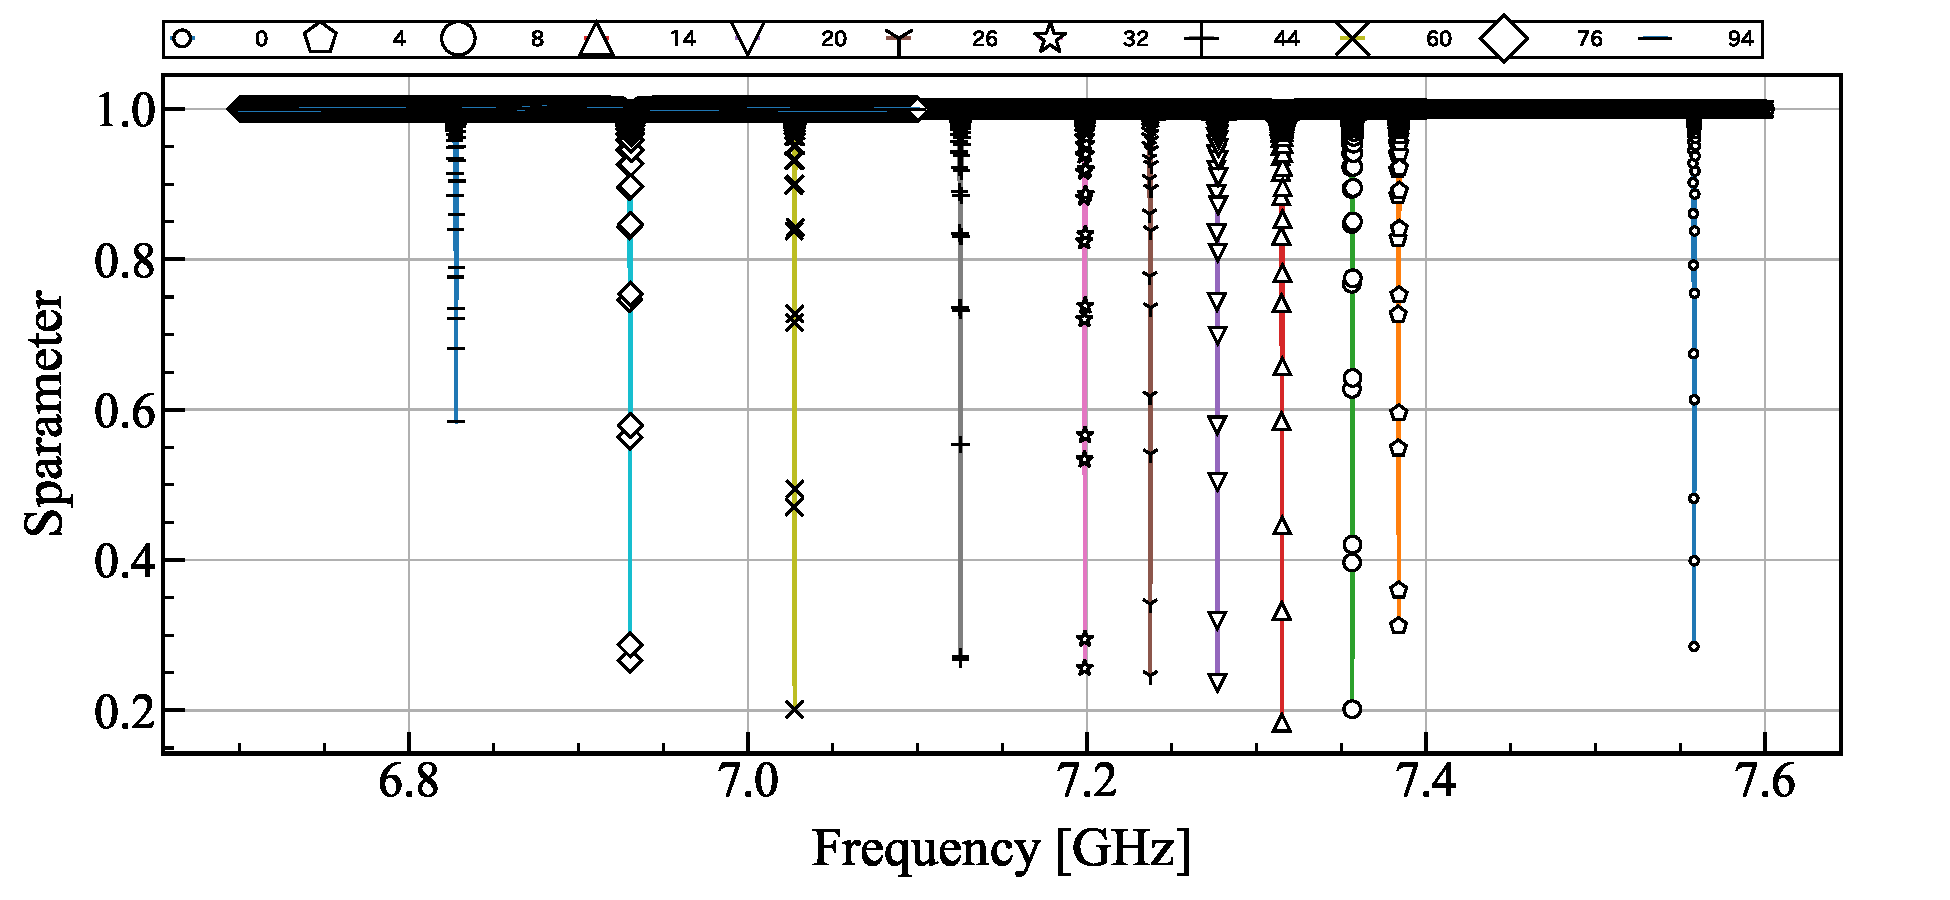
\includegraphics[width=12cm]{mwo_meander.pdf}
            \caption{dc-SQUIDによる$\beta$変調}
        \end{figure}
        電磁界シミュレータを用いてミアンダ(蛇行)の回数に対して共振器の周波数帯の変化をプロット下図をいかに示す。
        この各周波数デザインに対して低周波領域でシミュレーションを行うと回路全体のキャパシタンス、ミアンダインダクタンスがない場合との差分をとることでミアンダの回数に対してインダクタンスがどれだけ上昇するのかを見積もることができる。上記で示した解析的な手法とともにミアンダの回数に対するインダクタンスの値を示す。ここで固定している値はミアンダラインを構成している線路幅、及び折り返し幅である。
        \begin{figure}[H]
            \centering
            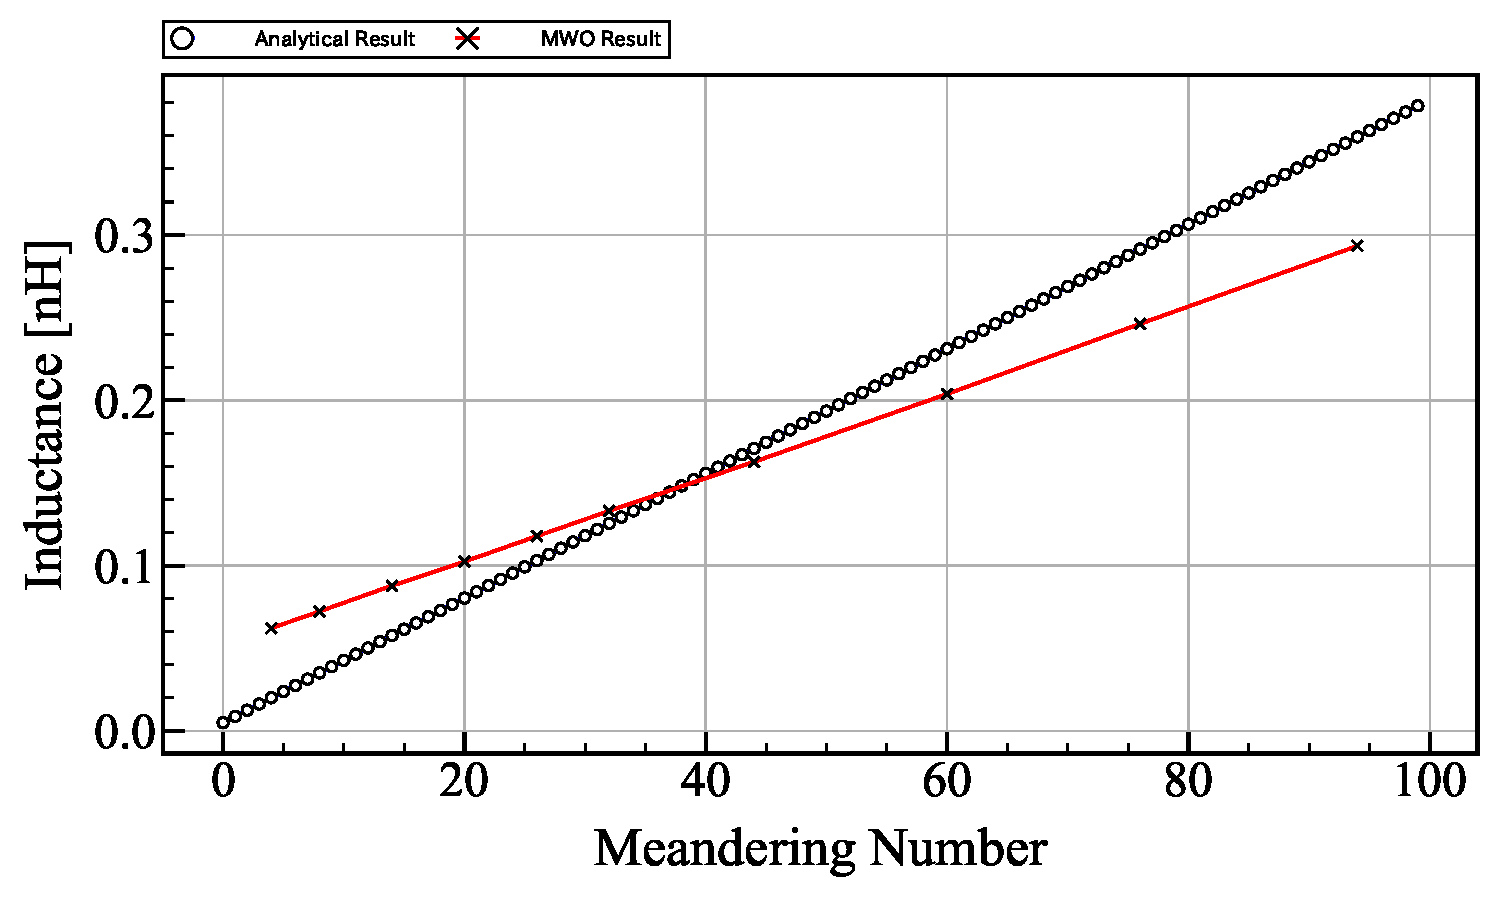
\includegraphics[width=12cm]{simulatorVSanalytical.pdf}
            \caption{Inductance VS Meandering Number}
        \end{figure}
        これによりシミュレータと解析的な計算によるミアンダインダクタンスには大きな差異はなかったことがわかる。本サンプルの設計にはミアンダの回数を38本に設定した。これは解析解とシミュレータに依る解が最も小さな本数を選んだ。また、インダクタンスが大きすぎると共振器間の距離にも依存するが、測定環境である4GHz~8GHz帯を逸脱してしまうため、外部磁場に依る遷移周波数の変化も考慮するとN=38本程度が妥当であるという帰結である。以下にN=38に置ける共振器埜パラメータを示す。
        \begin{figure}[H]
            \centering
            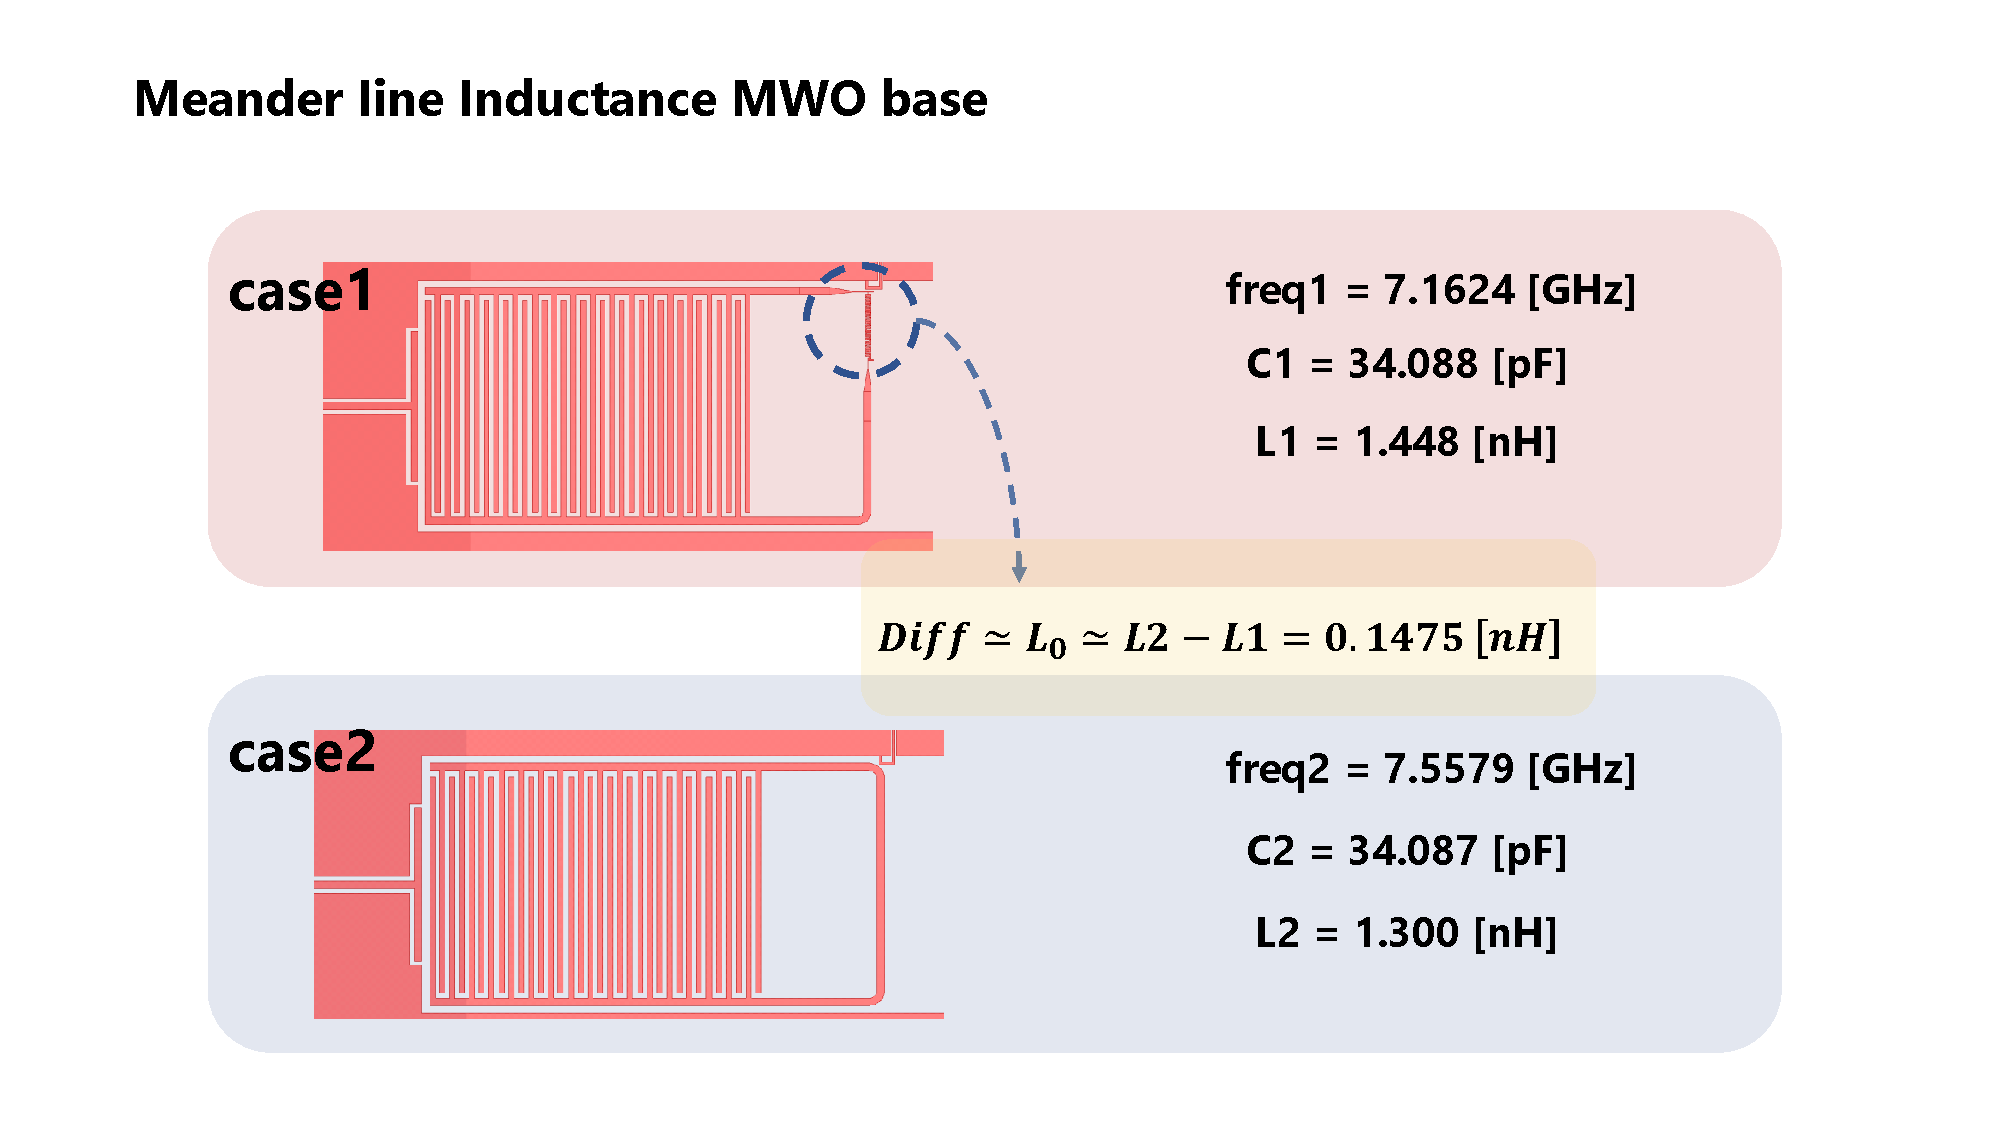
\includegraphics[width=12cm]{meanderinductance.pdf}
            \caption{電磁界シミュレーションによる導出}
        \end{figure}
        さて、作成したサンプルであるが、メインループとdc-SQUIDの面積比を100倍にすることで独立に操作できるようにしたと述べたが、実際にはどのような応答が得られるを示す。オンチップバイアスを固定した状態でグローバルバイアスを適当な値だけ駆動するとdc-SQUIDの応答をみることができる。
        \begin{figure}[H]
            \centering
            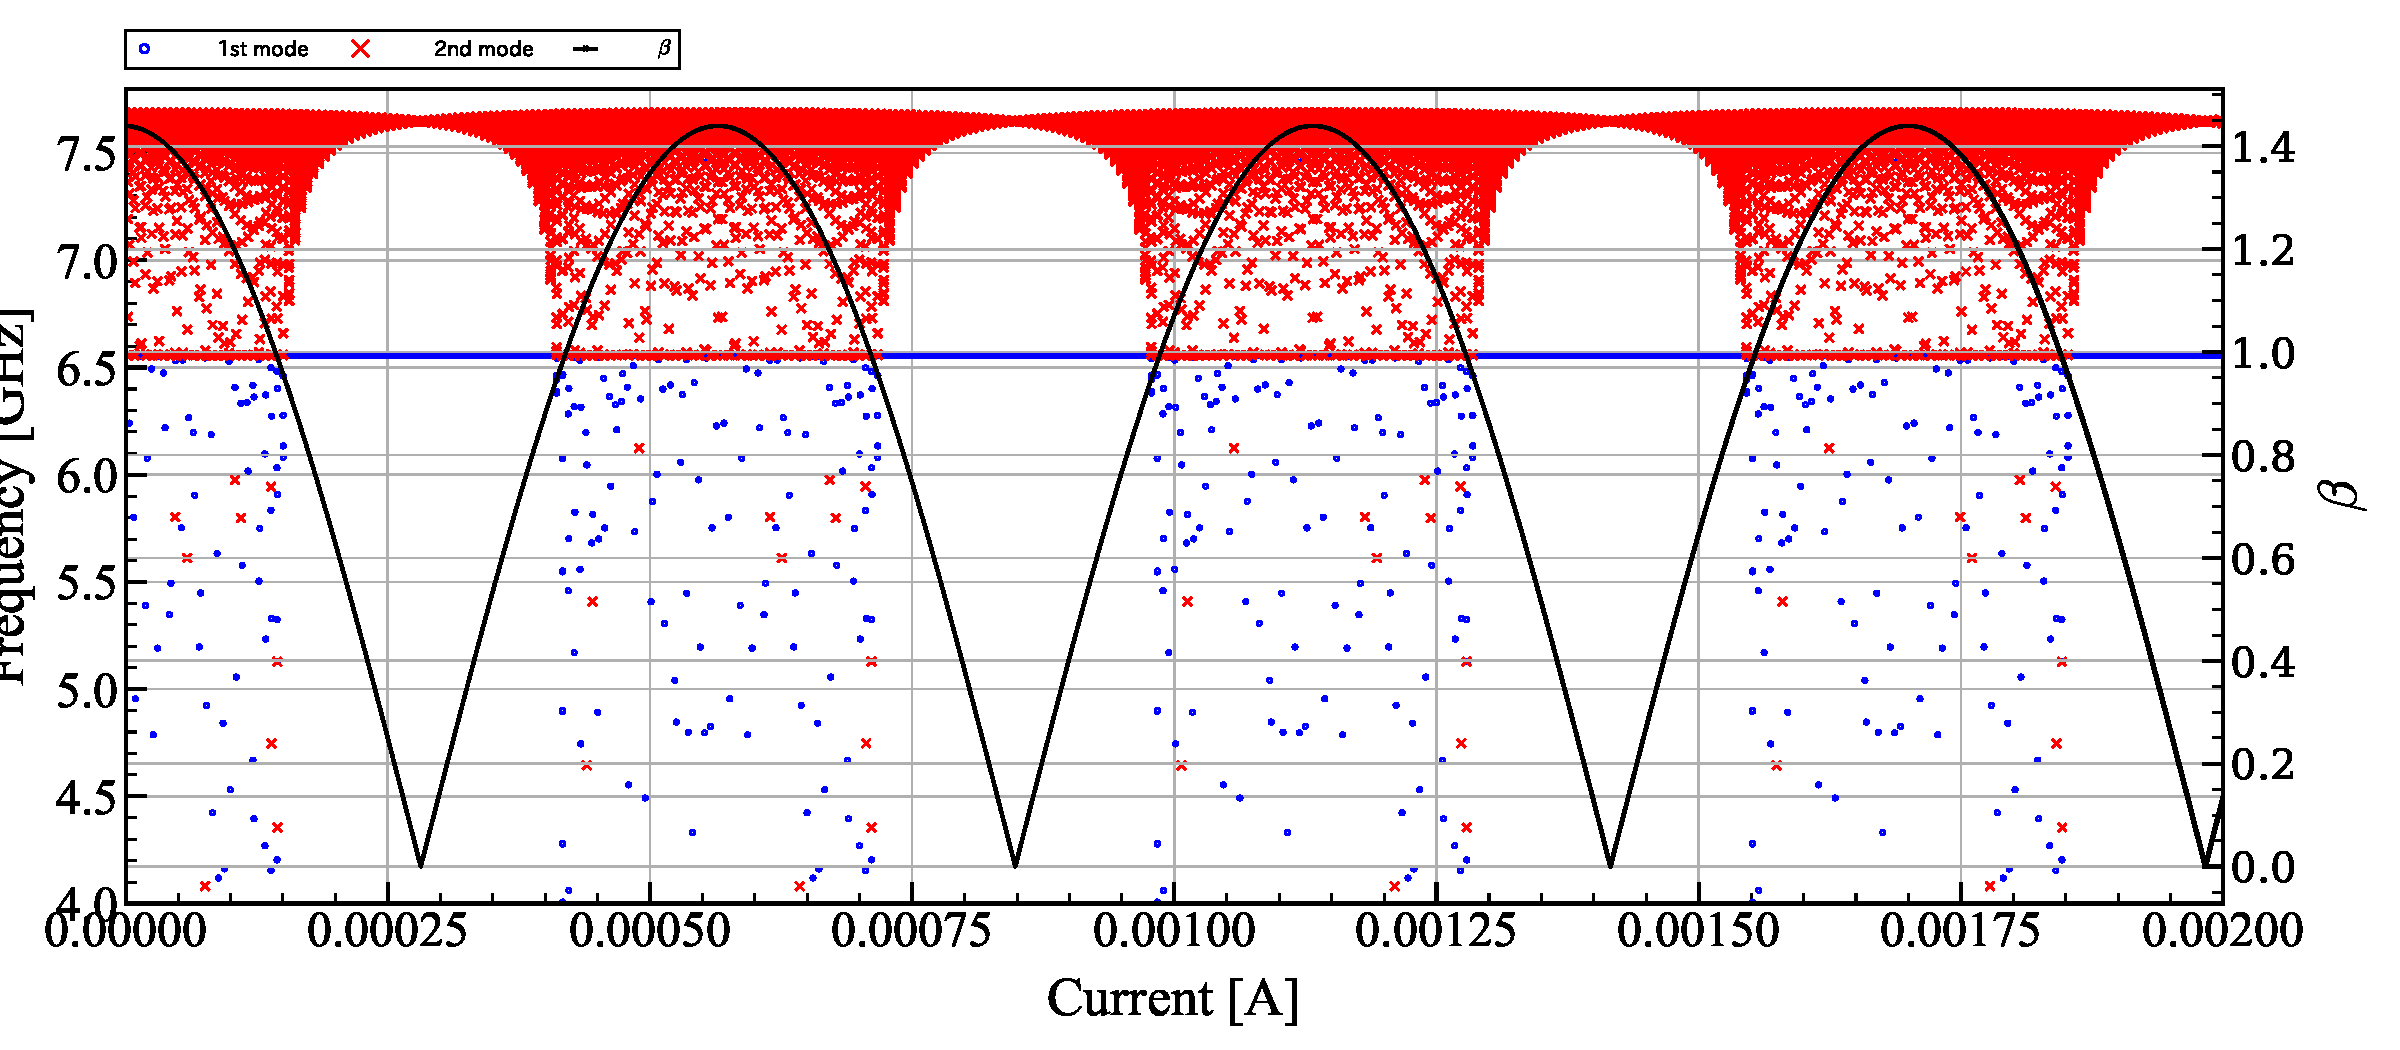
\includegraphics[width=12cm]{compound1.pdf}
            \caption{dc-SQUIDによる$\beta$変調}
        \end{figure}
        図中黒線がスクリーニングである。スクリーニングパラメータがゼロとなるとき、結合強度中
        \begin{equation}
            g(\Phi) = g0\frac{\beta cos(\Phi)}{1+\beta cos(\Phi)} + g1
        \end{equation}
        磁束依存項がゼロとなり、結合強度は共振器間の1次結合のみとなる。この時2つのモードは電磁界シミュレーションで計算した周波数帯に対応するシグナルとなる。測定ではこのシミュレーションと同じようにグローバルバイアスのみを駆動しスクリーニングパラメータの区間周期を見積もる。
        次にある点でグローバルバイアスを固定しオンチップバイアスのみを駆動する。これによスクリーニングパラメータを固定下状態で結合素子を操作することが可能となる。

\section{設計}
        以上の結果を用いて回路の設計を行う。本回路では共振器及び伝送線路をNbで、ジョセフソン接合を含む結合素子をAlで構成している。それぞれのデザインパターンをAutoDesk社のAutoCAD(ver2018)で作成する。以下に作成したデザインパターンを示す。Nb⇒Alという手順で製造する。Si基板にNbをスパッタし、電子線描画装置でデザインパターンを作成する。
    \subsection{製造パラメータ}

    \subsection{二重角度蒸着}

\section{測定サンプル}
    上記の計算により求めた設計値に基づいて作成したgdsファイルが以下である。
    \begin{figure}[H]
        \centering
        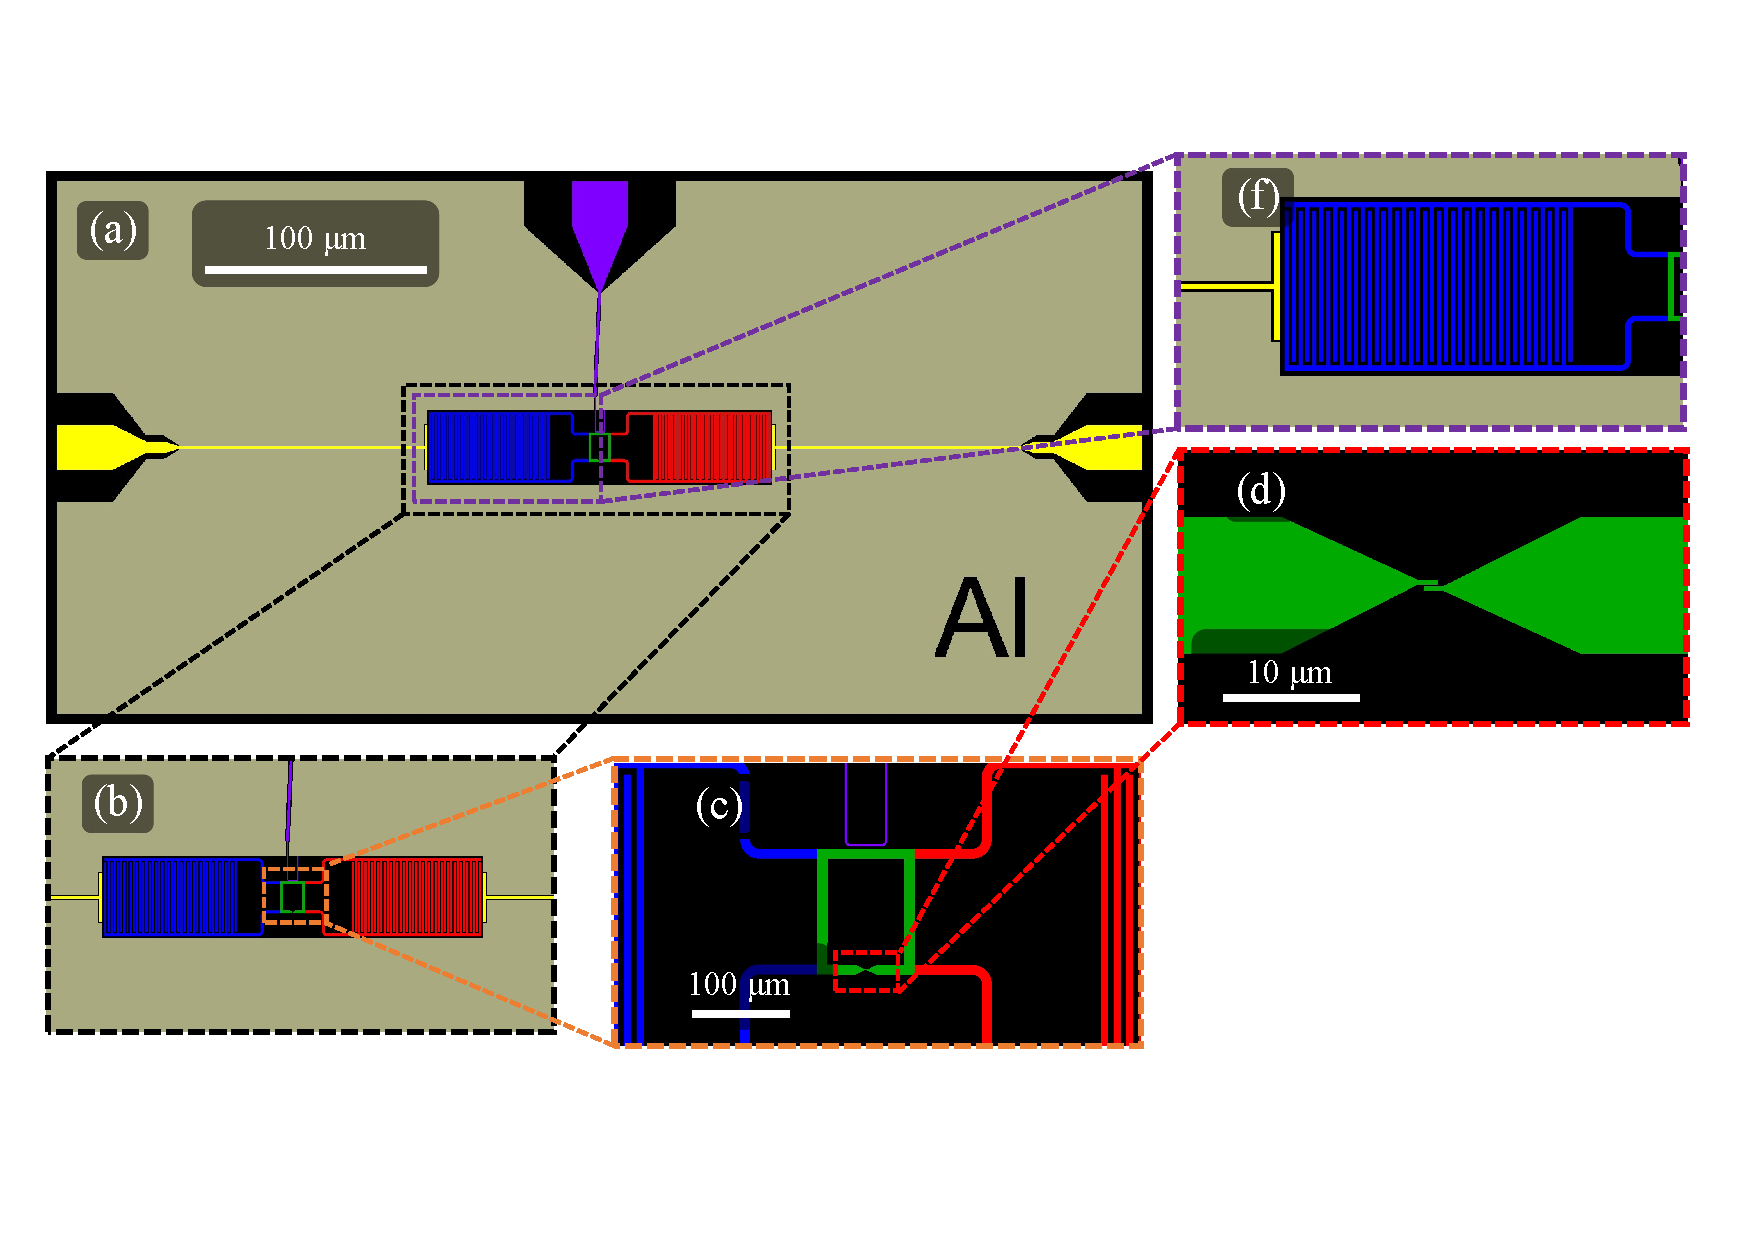
\includegraphics[width=14cm]{design1.pdf}
        \caption{LCC回路デザイン}
    \end{figure}

    \begin{figure}[H]
        \centering
        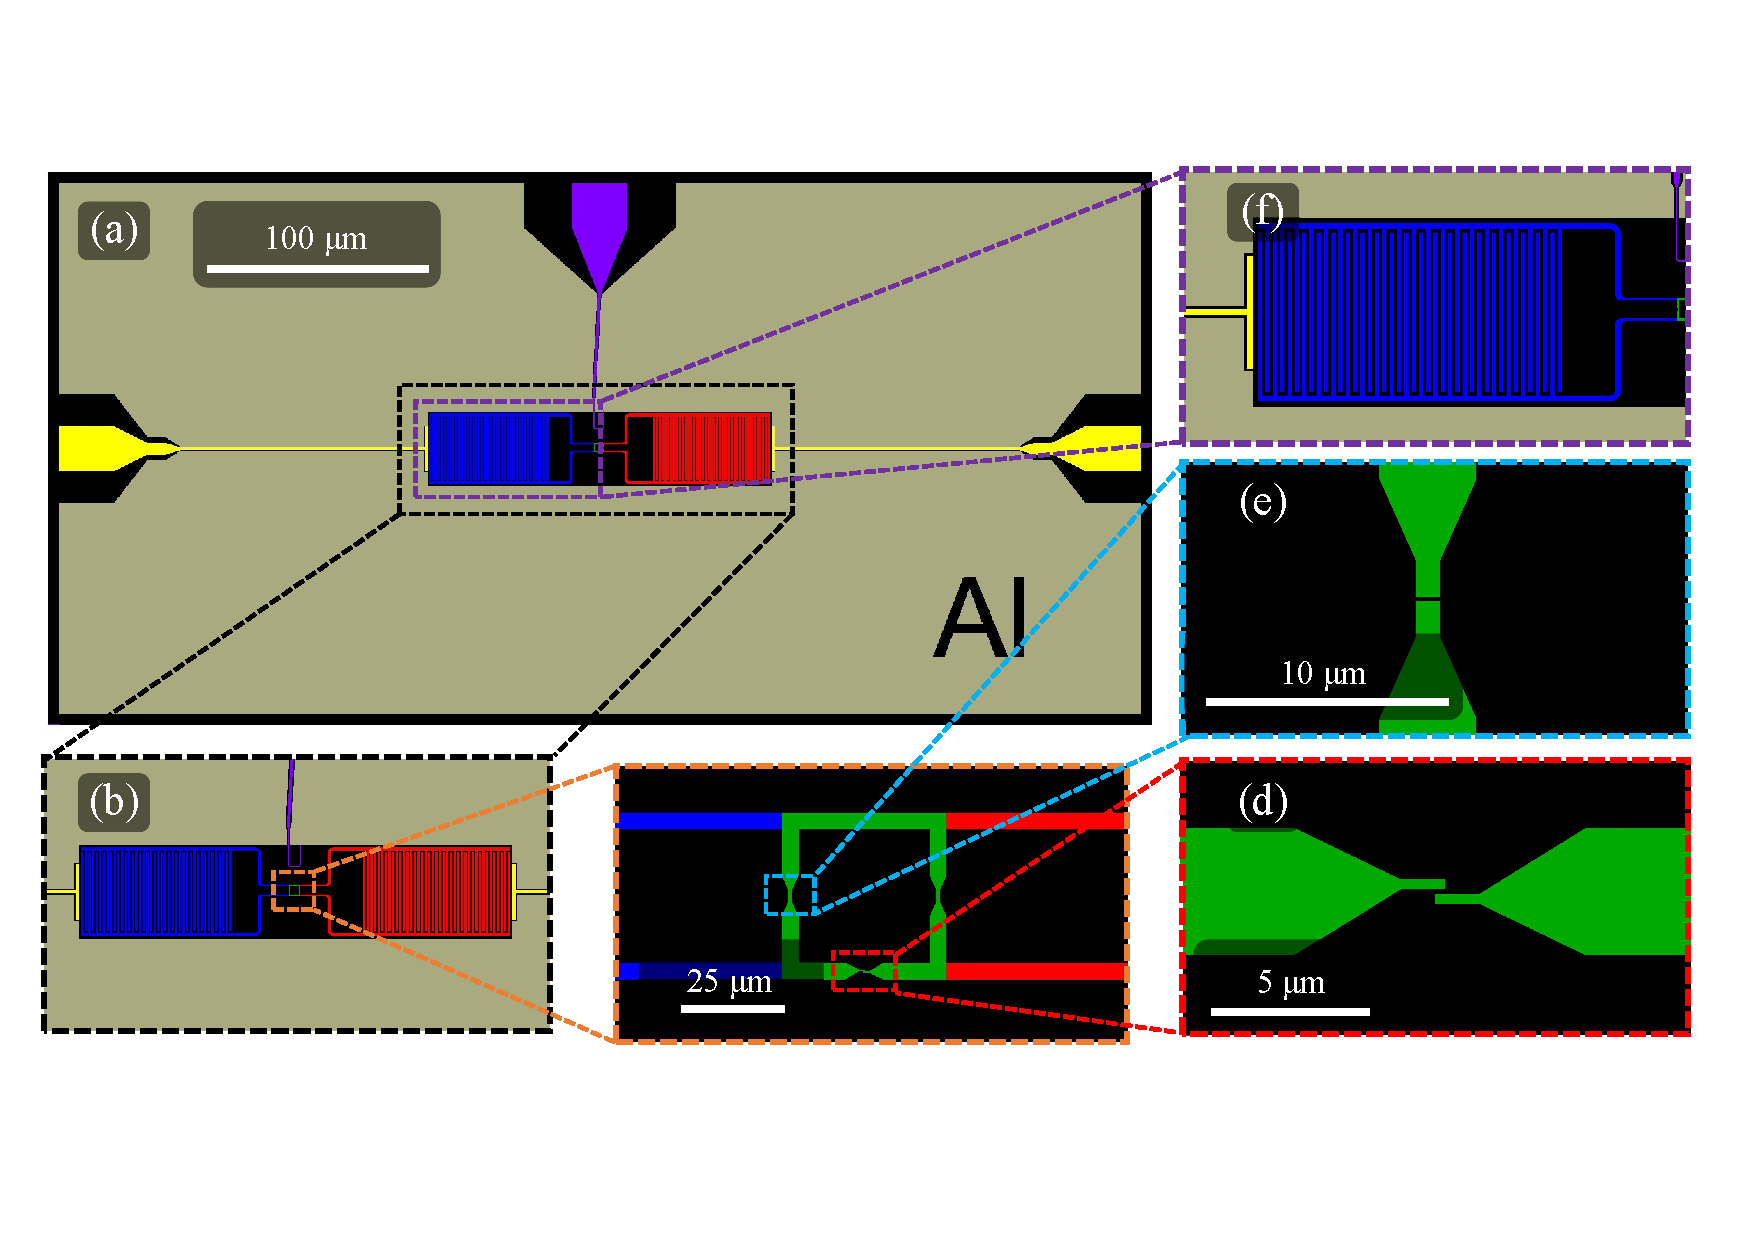
\includegraphics[width=14cm]{design2.pdf}
        \caption{JLCC回路デザイン}
    \end{figure}

    \begin{figure}[H]
        \centering
        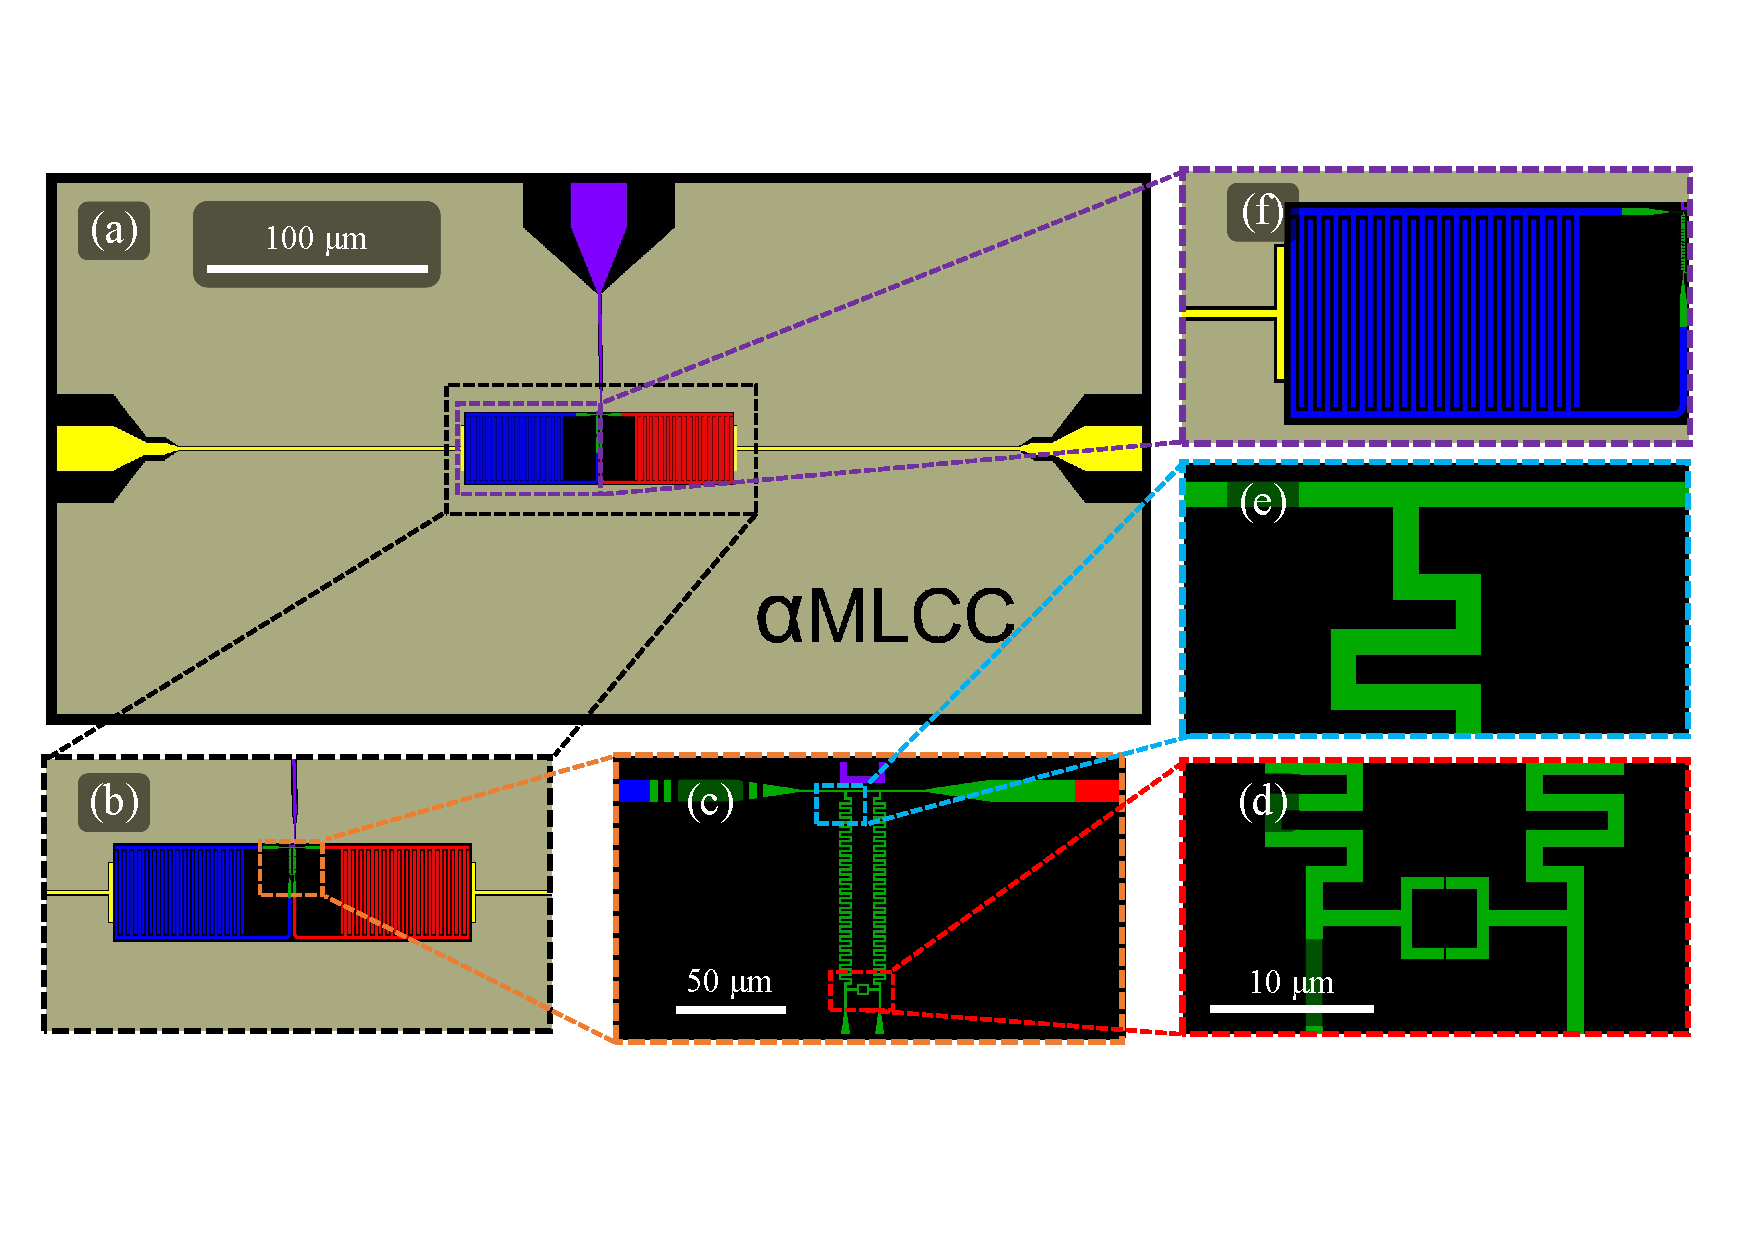
\includegraphics[width=14cm]{design3.pdf}
        \caption{aMLCC回路デザイン}
    \end{figure}
    \subsection{回路パラメータ}
